
%Este archivo no tiene contenido, mas allá de configuraciones y\o definiciones.
%todo el contenido se encuentra en los archivos secundarios que son importados por este.

\documentclass[twoside,letterpaper]{article}


%\\\\\\\\\\\\\\\\\\\\\\\\\\\
%Packages en uso

%Idiomas diccionario
\usepackage[english, spanish]{babel}
%\usepackage[english]{babel}

\usepackage[utf8x]{inputenc}
%\usepackage[latin1]{inputenc} 
%\usepackage[ansinew]{inputenc}
\usepackage{ucs}




%\usepackage[margin=1cm, paperwidth=21.0cm, paperheight=29.6cm]{geometry}



\usepackage[T1]{fontenc} 
\usepackage{graphicx}
\usepackage{float}
\usepackage{longtable}
%\usepackage{floatflt}
\usepackage{fancyhdr}
\usepackage{hyperref}
%\usepackage{url}
\usepackage{amsfonts}
\usepackage{amssymb}
\usepackage{textcomp}
%\usepackage[symbol]{footmisc}
%\usepackage{pst-circ}
%\usepackage{epsfig}
%\usepackage{xkeyval}
\usepackage{tabularx}
\usepackage{booktabs}


%\usepackage{color}
\usepackage[usenames,dvipsnames]{color}


%\usepackage{minted}
\usepackage{latexsym}
\usepackage{colortbl}
%\usepackage{pdfpages}
\usepackage{wrapfig}

%\usepackage{listings}
\usepackage{listingsutf8}
%\usepackage{mips}
\usepackage{appendix}
\usepackage{needspace}
\usepackage{ifplatform}
\usepackage{ifthen}



%\\\\\\\\\\\\\\\\\\\\\\\\\\\
% FOR GNUPLOT
%\usepackage{tikz}

%\usepackage[miktex]{gnuplottex}
%\usepackage{gnuplot-lua-tikz}
%\usepackage{mathpazo}
%\\\\\\\\\\\\\\\\\\\\\\\\\\\


%\\\\\\\\\\\\\\\\\\\\\\\\\\\
% FOR FIGURE CAPTION COLORS

\usepackage{caption}
\usepackage[svgnames]{xcolor}

%\\\\\\\\\\\\\\\\\\\\\\\\\\\

%\\\\\\\\\\\\\\\\\\\\\\\\\\\
% FOR FIGURE WRAPPING

\usepackage{wrapfig}

%\\\\\\\\\\\\\\\\\\\\\\\\\\\


%\\\\\\\\\\\\\\\\\\\\\\\\\\\
% FOR EQUATION CAPTION FORMAT, COLORS AND OTHERS

\usepackage{amsmath}
\usepackage{mathtools}
\usepackage{bm}

%\\\\\\\\\\\\\\\\\\\\\\\\\\\


%\\\\\\\\\\\\\\\\\\\\\\\\\\\
% TABLES

\usepackage{makecell, multirow, tabularx}
    \newcolumntype{L}{>{\raggedright\arraybackslash}X}
    \renewcommand\theadfont{\normalsize\bfseries\color{white}}
\usepackage{hhline}
\usepackage{setspace}

%\\\\\\\\\\\\\\\\\\\\\\\\\\\


%\\\\\\\\\\\\\\\\\\\\\\\\\\\
% UNITS

\usepackage{siunitx}

\sisetup{output-exponent-marker=\ensuremath{\mathrm{e}}}

%\\\\\\\\\\\\\\\\\\\\\\\\\\\


%\\\\\\\\\\\\\\\\\\\\\\\\\\\
% MATH

\usepackage{mathrsfs}

\usepackage{mathtools}

\usepackage{amsmath,mleftright}

\usepackage{xparse}

\numberwithin{equation}{subsection}

\NewDocumentCommand{\evalat}{sO{\big}mm}{%
  \IfBooleanTF{#1}
   {\mleft. #3 \mright|_{#4}}
   {#3#2|_{#4}}%
}

%\\\\\\\\\\\\\\\\\\\\\\\\\\\

%\\\\\\\\\\\\\\\\\\\\\\\\\\\
%!!!!!!!!!!!!!!!!!!!!!!!!! DETECCION DE PLATAFORMA !!!!!!!!!!!!!!!!!!!!!!!!!!!!!!!!!
%Permite que sea compilado tanto en windows como en *IX sin cambio alguno.
\newboolean{IsWindows}
\ifwindows
\setboolean{IsWindows}{true}
\else
\setboolean{IsWindows}{false}
\fi
%\\\\\\\\\\\\\\\\\\\\\\\\\\\
%!!!!!!!!!!!!!!!!!!!!!!!!!!!!!!!!!!!!!!!!!!!!!!!!!!!!!!!!!!!!!!!!!!!!!!!!!!!!!!!!!!!!

%\\\\\\\\\\\\\\\\\\\\\\\\\\\
%Idiomas
\hyphenrules{spanish}
%\\\\\\\\\\\\\\\\\\\\\\\\\\\


%\\\\\\\\\\\\\\\\\\\\\\\\\\\
%Comandos personalizados

\newcommand{\titulo}{Trabajo práctico N\textdegree \hspace{1pt} 1}
\newcommand{\titulolargo}{Análisis de amplificador clase B}
\newcommand{\materia}{Seminario de Audio Profesional - 66.66}
\newcommand{\fiuba}{Facultad de Ingeniería - UBA}
\newcommand{\cuatrimestre}{1\textsuperscript{er} c. 2020} %\sptext{do} $2^{do}$



\newcommand{\autorA}{\textsc{Luna} Diego}
\newcommand{\padronA}{75451}
\newcommand{\mailA}{\weblink{mailto:diegorluna@gmail.com}{diegorluna@gmail.com}} 
 
 
 
\newcommand{\docenteA}{Ing. \textsc{Sinnewald} Daniel Nestor}
\newcommand{\docenteB}{Ing. \textsc{Rubinstein} Lucas Tomás}



\newcommand{\thedate}{7 de Junio de 2020}


\newcommand{\HRule}{\rule{\linewidth}{0.3mm}}

%\\\\\\\\\\\\\\\\\\\\\\\\\\\


%\\\\\\\\\\\\\\\\\\\\\\\\\\\
%Título,  autor del documento y fecha
\title{\titulo}
\author{\autorB}
\date{\thedate}
%\\\\\\\\\\\\\\\\\\\\\\\\\\\


%\\\\\\\\\\\\\\\\\\\\\\\\\\\
\setcounter{secnumdepth}{5}
\setcounter{tocdepth}{5}
%\\\\\\\\\\\\\\\\\\\\\\\\\\\


%\\\\\\\\\\\\\\\\\\\\\\\\\\\
%suppress widows and orphans
\widowpenalty=9999
\clubpenalty=9999
%\\\\\\\\\\\\\\\\\\\\\\\\\\\


%\\\\\\\\\\\\\\\\\\\\\\\\\\\
%equation numbers to subsection level
%\numberwithin{equation}{subsection}
\numberwithin{equation}{section}
%\\\\\\\\\\\\\\\\\\\\\\\\\\\


%\\\\\\\\\\\\\\\\\\\\\\\\\\\
%equation numbers to subsection level
%\numberwithin{table}{subsection}
\numberwithin{table}{section}
%\\\\\\\\\\\\\\\\\\\\\\\\\\\



%\\\\\\\\\\\\\\\\\\\\\\\\\\\
%figure numbers to subsection level
%\renewcommand{\thefigure}{\thesubsection.\arabic{figure}}
\renewcommand{\thefigure}{\thesection.\arabic{figure}}
%\\\\\\\\\\\\\\\\\\\\\\\\\\\

%\setlength{\arrayrulewidth}{0.6pt}


%\\\\\\\\\\\\\\\\\\\\\\\\\\\
\newcolumntype{z}[1]{%
>{\centering\hspace{0pt}}p{#1}}%

\newcolumntype{y}[1]{%
>{\raggedleft\hspace{0pt}}p{#1}}% 

\newcolumntype{x}[1]{%
>{\raggedright\hspace{0pt}}p{#1}}% 

\newcolumntype{w}[1]{%
>{\centering\hspace{0pt}}m{#1}}%

\newcolumntype{v}[1]{%
>{\raggedleft\hspace{0pt}}m{#1}}% 

\newcolumntype{u}[1]{%
>{\raggedright\hspace{0pt}}m{#1}}% 


\newcommand{\tn}{\tabularnewline}
%\\\\\\\\\\\\\\\\\\\\\\\\\\\




%\\\\\\\\\\\\\\\\\\\\\\\\\\\
% Generales
\newcommand{\quotemarks}[1]{``#1''}
\newcommand{\simplequotemarks}[1]{`#1'}
%\\\\\\\\\\\\\\\\\\\\\\\\\\\


%\\\\\\\\\\\\\\\\\\\\\\\\\\\
% Símbolos de las unidades

%\newcommand{\volt}[1]{\mbox{#1 V}}
%\newcommand{\milivolt}[1]{\mbox{#1 mV}}
%\newcommand{\hertz}[1]{\mbox{#1 Hz}}
%\newcommand{\kilohertz}[1]{\mbox{#1 kHz}}
%\newcommand{\megahertz}[1]{\mbox{#1 MHz}}
%\newcommand{\farad}[1]{\mbox{#1 F}}
%\newcommand{\nanofarad}[1]{\mbox{#1 nF}}
%\newcommand{\microfarad}[1]{\mbox{#1 $\mu$F}}
%\newcommand{\picofarad}[1]{\mbox{#1 pF}}
%\newcommand{\fentofarad}[1]{\mbox{#1 fF}}
%\newcommand{\ohm}[1]{\mbox{#1 $\Omega$}}
%\newcommand{\miliohm}[1]{\mbox{#1 m$\Omega$}}
%\newcommand{\kiloohm}[1]{\mbox{#1 k$\Omega$}}
%\newcommand{\megaohm}[1]{\mbox{#1 M$\Omega$}}
%\newcommand{\amper}[1]{\mbox{#1 A}}
%\newcommand{\miliamper}[1]{\mbox{#1 mA}}
%\newcommand{\microamper}[1]{\mbox{#1 $\mu$A}}
%\newcommand{\picoamper}[1]{\mbox{#1 pA}}
%\newcommand{\fentoamper}[1]{\mbox{#1 fA}}
%\newcommand{\s}[1]{\mbox{#1 s}}
%\newcommand{\milis}[1]{\mbox{#1 ms}}
%\newcommand{\micros}[1]{\mbox{#1 $\mu$s}}
%\newcommand{\nanos}[1]{\mbox{#1 ns}}
%\newcommand{\miliamperporvolt}[1]{ \mbox{#1 $\frac{mA}{V}$}}
%\newcommand{\miliamperporvoltcuad}[1]{ \mbox{#1 $\frac{mA}{V^2}$}}
%\newcommand{\decibel}[1]{\mbox{#1 dB}}
%\newcommand{\decibeli}[1]{\mbox{#1 dBi}}


% Nombres de las unidades
%\newcommand{\Metro}{\mbox{metro}}
%\newcommand{\Volt}{\mbox{Volt}}
%\newcommand{\Amper}{\mbox{Ampere}}
%\newcommand{\Farad}{\mbox{Farad}}

\newcommand{\spice}{\mbox{\textit{\textbf{SPICE}}}}
\newcommand{\schematic}{\mbox{\textit{\textbf{SCHEMATIC}}}}

\newcommand{\parallelresistors}{\mathbin{\!/\mkern-5mu/\!}}


%\\\\\\\\\\\\\\\\\\\\\\\\\\\

%\\\\\\\\\\\\\\\\\\\\\\\\\\\
% Dispositivos

\newcommand{\mosfet}{\mbox{\textbf{MOSFET}}}
\newcommand{\nmosfet}{\mbox{\textbf{NMOSFET}}}
\newcommand{\bjtnpn}{\mbox{\textbf{BJT NPN}}}
\newcommand{\bjtpnp}{\mbox{\textbf{BJT PNP}}}

%\\\\\\\\\\\\\\\\\\\\\\\\\\\

%\\\\\\\\\\\\\\\\\\\\\\\\\\\
% Plataformas

\newcommand{\platformhost}{\textbf{x86(\_64)\textbackslash Linux}}
\newcommand{\platformguest}{\textbf{pmax\textbackslash NetBSD}}

\newcommand{\oshost}{\textbf{Linux}}
\newcommand{\osguest}{\textbf{NetBSD}}

\newcommand{\MIPS}{\textbf{MIPS32}}
%\\\\\\\\\\\\\\\\\\\\\\\\\\\


%\\\\\\\\\\\\\\\\\\\\\\\\\\\
% Programación

\newcommand{\GNU}{\textbf{GNU}}

\newcommand{\GCC}{\textbf{GCC}}

\newcommand{\GDB}{\textbf{GDB}}

\newcommand{\GXEMUL}{\textbf{GXemul}}

\newcommand{\langc}{\textbf{\quotemarks{C}}}

\newcommand{\langass}{\textbf{assembly}}

\newcommand{\langmipsass}{\textbf{MIPS32 assembly}}

\newcommand{\make}{\textbf{make}}
%\\\\\\\\\\\\\\\\\\\\\\\\\\\


%\\\\\\\\\\\\\\\\\\\\\\\\\\\
% Archivos

\newcommand{\quotefile}[1]{\textit{\quotemarks{#1}}}

\newcommand{\filebox}[2]{%

\begin{tabular}{l}

\multicolumn{1}{>{\columncolor{#2}}l}{#1} 
	
\end{tabular}

}%
%\\\\\\\\\\\\\\\\\\\\\\\\\\\



%\\\\\\\\\\\\\\\\\\\\\\\\\\\
% Math
\newcommand{\Reales}{\mathbb{R}}
\newcommand{\Complejos}{\mathbb{C}}
\newcommand{\numnorm}[1]{\left|#1\right|}
\newcommand{\vectornorm}[1]{\left|\left|#1\right|\right|}
%\\\\\\\\\\\\\\\\\\\\\\\\\\\


%\\\\\\\\\\\\\\\\\\\\\\\\\\\
% Counters
\newcommand{\resetallcounters}{%
\setcounter{figure}{0}
\setcounter{equation}{0}
\setcounter{table}{0}
}%
%\\\\\\\\\\\\\\\\\\\\\\\\\\\



%\\\\\\\\\\\\\\\\\\\\\\\\\\\
% Definiciones de colores.
\definecolor{Deepblue}{rgb}{0.00,0.00,0.70}
\definecolor{Deepgreen}{rgb}{0.09,0.45,0.20}
\definecolor{Darkgreen}{RGB}{0, 128, 0}
\definecolor{Purple}{rgb}{1,0,1}
\definecolor{Deeppurple}{rgb}{0.2,0,1}
\definecolor{Gray}{rgb}{0.3,0.3,0.3}
\definecolor{Lightblue}{rgb}{0.60, 0.80, 1.00}
\definecolor{Lightyellow}{rgb}{1.00,1.00,0.60}
\definecolor{LightButter}{rgb}{0.98,0.91,0.31}
\definecolor{LightOrange}{rgb}{0.98,0.68,0.24}
\definecolor{LightChocolate}{rgb}{0.91,0.72,0.43}
\definecolor{LightChameleon}{rgb}{0.54,0.88,0.20}
\definecolor{LightSkyBlue}{rgb}{0.45,0.62,0.81}
\definecolor{LightPlum}{rgb}{0.68,0.50,0.66}
\definecolor{LightScarletRed}{rgb}{0.93,0.16,0.16}
\definecolor{Butter}{rgb}{0.93,0.86,0.25}
\definecolor{Orange}{rgb}{0.96,0.47,0.00}
\definecolor{Chocolate}{rgb}{0.75,0.49,0.07}
\definecolor{Chameleon}{rgb}{0.45,0.82,0.09}
\definecolor{SkyBlue}{rgb}{0.20,0.39,0.64}
\definecolor{Plum}{rgb}{0.46,0.31,0.48}
\definecolor{ScarletRed}{rgb}{0.80,0.00,0.00}
\definecolor{DarkButter}{rgb}{0.77,0.62,0.00}
\definecolor{DarkOrange}{rgb}{0.80,0.36,0.00}
\definecolor{DarkChocolate}{rgb}{0.56,0.35,0.01}
\definecolor{DarkChameleon}{rgb}{0.30,0.60,0.02}
\definecolor{DarkSkyBlue}{rgb}{0.12,0.29,0.53}
\definecolor{DarkPlum}{rgb}{0.36,0.21,0.40}
\definecolor{DarkScarletRed}{rgb}{0.64,0.00,0.00}
\definecolor{Aluminium1}{rgb}{0.93,0.93,0.92}
\definecolor{Aluminium2}{rgb}{0.82,0.84,0.81}
\definecolor{Aluminium3}{rgb}{0.73,0.74,0.71}
\definecolor{Aluminium4}{rgb}{0.53,0.54,0.52}
\definecolor{Aluminium5}{rgb}{0.33,0.34,0.32}
\definecolor{Aluminium6}{rgb}{0.18,0.20,0.21}

\definecolor{EQColor}{rgb}{0.00,0.26,0.36} % {0.80,0.36,0.00}
\definecolor{FIGColor}{cmyk}{1,0.00,0.00,0.00}
\definecolor{TABLEColor}{RGB}{199,25,0}



\definecolor{APENDLINKColor}{rgb}{0.96,0.47,0.00}
\definecolor{SECTLINKColor}{rgb}{1.00,0.30,0.00}
\definecolor{FILELINKColor}{rgb}{1.00,0.00,0.00}
\definecolor{INTERNALLINKColor}{rgb}{1.00,0.00,0.00}
\definecolor{WEBLINKColor}{rgb}{0.00,0.00,1.00}
\definecolor{CITELINKColor}{RGB}{141,199,126}
\definecolor{TABLELINKColor}{RGB}{199,25,0}


%\definecolor{EQColor}{rgb}{0.00,0.36,0.80}
%\definecolor{FIGColor}{cmyk}{1,0.00,0.00,0.00}
%\definecolor{TABLEColor}{RGB}{0,199,25}



%\definecolor{APENDLINKColor}{rgb}{0.10,0.47,0.00}
%\definecolor{SECTLINKColor}{rgb}{0.00,0.00,1.00}
%\definecolor{FILELINKColor}{rgb}{0.00,0.00,1.00}
%\definecolor{INTERNALLINKColor}{rgb}{0.00,0.00,1.00}
%\definecolor{WEBLINKColor}{rgb}{0.00,0.00,1.00}
%\definecolor{CITELINKColor}{RGB}{141,199,126}
%\definecolor{TABLELINKColor}{RGB}{199,199,0}


\definecolor{HeadersColor}{RGB}{0,137,182}

%\\\\\\\\\\\\\\\\\\\\\\\\\\\


%\\\\\\\\\\\\\\\\\\\\\\\\\\\
% FOR FIGURE CAPTION COLORS

\DeclareCaptionFont{FIGFont}{\color{FIGColor}}
\captionsetup[figure]{labelfont={FIGFont,bf}}

\newcommand{\figref}[1]{\textcolor{FIGColor}{[\ref{#1}]}}
%\\\\\\\\\\\\\\\\\\\\\\\\\\\


%\\\\\\\\\\\\\\\\\\\\\\\\\\\
% FOR TABLE CAPTION COLORS

\DeclareCaptionFont{TABLEFont}{\color{TABLEColor}}
\captionsetup[table]{labelfont={TABLEFont,bf}}

\newcommand{\tableref}[1]{\textcolor{TABLEColor}{[\ref{#1}]}}


%\captionsetup[table]{style=fortables}
%\captionsetup[figure]{style=forfigures}
%\\\\\\\\\\\\\\\\\\\\\\\\\\\


%\\\\\\\\\\\\\\\\\\\\\\\\\\\
% FOR EQUATION CAPTION FORMAT, COLORS AND OTHERS

\newtagform{brackets2}[\textcolor{EQColor}]{\textcolor{EQColor}(}{\textcolor{EQColor})}
\usetagform{brackets2}

%\\\\\\\\\\\\\\\\\\\\\\\\\\\


%\\\\\\\\\\\\\\\\\\\\\\\\\\\
% FOR EQUATION CAPTION COLORS
%\makeatletter %% Without ams
%\def\@eqnnum{{\normalfont\normalcolor[\theequation]}}
%\makeatother

%But amsmath redefines the numbering of equations, so then you can do:

%\makeatletter %% With ams
%\def\tagform@#1{\maketag@@@{[\ignorespaces#1\unskip\@@italiccorr]}}
%\makeatother 
%\\\\\\\\\\\\\\\\\\\\\\\\\\\


%\\\\\\\\\\\\\\\\\\\\\\\\\\\
% FOR APENDIX REFERENCE

\newcommand{\apendref}[1]{\textcolor{APENDLINKColor}{[\ref{#1}]}}

%\\\\\\\\\\\\\\\\\\\\\\\\\\\


%\\\\\\\\\\\\\\\\\\\\\\\\\\\
% FOR SECTION REFERENCE

\newcommand{\sectref}[1]{\textcolor{SECTLINKColor}{[\ref{#1}]}}

%\\\\\\\\\\\\\\\\\\\\\\\\\\\


%\\\\\\\\\\\\\\\\\\\\\\\\\\\
% WEB LINK

\newcommand{\weblink}[2]{\href{#1}{\textcolor{WEBLINKColor}{#2}}}

%\\\\\\\\\\\\\\\\\\\\\\\\\\\


%\\\\\\\\\\\\\\\\\\\\\\\\\\\
% FILE LINK

\newcommand{\filelink}[2]{\href{#1}{\textcolor{FILELINKColor}{#2}}}

%\\\\\\\\\\\\\\\\\\\\\\\\\\\


%\\\\\\\\\\\\\\\\\\\\\\\\\\\
% CITE LINK
\newcommand{\citelink}[1]{\textcolor{LimeGreen}{\cite{#1}}}

%\\\\\\\\\\\\\\\\\\\\\\\\\\\


\hypersetup{
%	bookmarksnumbered,
%	pdfpagemode={UseOutlines},
%    bookmarks=true,         				% show bookmarks bar?
    unicode=true,          					% non-Latin characters in Acrobat’s bookmarks
    pdftoolbar=true,        				% show Acrobat’s toolbar?
    pdfmenubar=true,        				% show Acrobat’s menu?
%    pdffitwindow=false,    				% window fit to page when opened
%    pdfstartview={FitH},   				% fits the width of the page to the window
    pdftitle={\titulo},   					% title
    pdfauthor={\autorA},    				% author
    pdfsubject={\materia},   				% subject of the document
%    pdfcreator={\LaTeX},   				% creator of the document
%    pdfproducer={Producer},				% producer of the document
    pdfkeywords={TL} {TP}, 					% list of keywords
    pdfnewwindow=true,      				% links in new window
    linktoc=all,							%
    colorlinks=false,  						% false: boxed links; true: colored links	
	linkcolor=INTERNALLINKColor,			% color of internal links
    citecolor=CITELINKColor,    			% color of links to bibliography
    filecolor=FILELINKColor,   	 			% color of file links
    urlcolor=WEBLINKColor,       			% color of external links	
	linkbordercolor=INTERNALLINKColor,		% color of internal links
	citebordercolor=CITELINKColor,			% color of links to bibliography
    filebordercolor=FILELINKColor,    		% color of file links
    urlbordercolor=WEBLINKColor}	       	% color of external links	    
   				
	


%\\\\\\\\\\\\\\\\\\\\\\\\\\\
%Comportamiento de los links a archivos externos.
%\hypersetup{pdfnewwindow=true}
%\\\\\\\\\\\\\\\\\\\\\\\\\\\

%\\\\\\\\\\\\\\\\\\\\\\\\\\\
%Tamaños de la página y margenes

\linespread{1.3}
\oddsidemargin .1cm
\evensidemargin .1cm
\textwidth 16.5cm
\topmargin 0in
\voffset = 0pt
\textheight 21.08cm %8.3in
%\\\\\\\\\\\\\\\\\\\\\\\\\\\



%\pagestyle{fancy}


%\\\\\\\\\\\\\\\\\\\\\\\\\\\
%Encabezado y pie de páginas para todas las páginas normales

\fancypagestyle{allpages}{%

\fancyhf{}  

\renewcommand{\headrulewidth}{0.4pt}
\renewcommand{\footrulewidth}{0.4pt}

%No convierte a mayúscula los nombres de capítulo y sección 
%ni muestra el número.
%\renewcommand{\chaptermark}[1]{}
\renewcommand{\sectionmark}[1]{\markright{##1}{}}
\renewcommand{\subsectionmark}[1]{}
\renewcommand{\subsubsectionmark}[1]{}


\setlength{\headheight}{12pt}

   
%\fancyhf[LOH,REH]{\fiuba}
%\fancyhf[ROH,LEH]{\titulo}

\fancyhf[LH]{\small{\fiuba}}
\fancyhf[CH]{\small{\materia}}
\fancyhf[RH]{\titulo} 

\fancyhf[LOF,REF]{\small{\cuatrimestre}}
\fancyhf[CF]{\small{\rightmark}}
\fancyhf[LEF, ROF]{\textbf{\thepage}} 

}

%\\\\\\\\\\\\\\\\\\\\\\\\\\\


%\\\\\\\\\\\\\\\\\\\\\\\\\\\
%Encabezado y pie de páginas para el índice
\fancypagestyle{indexstyle}{%

\fancyhf{} % clear all header and footer fields

\renewcommand{\headrulewidth}{0.4pt}
\renewcommand{\footrulewidth}{0.4pt}

\setlength{\headheight}{12pt}


\fancyhf[LH]{
\includegraphics[width=3cm]{./img/logo_encabezado_fiuba}}
\fancyhf[CH]{\small{\materia}}
\fancyhf[RH]{\titulo}

\fancyhf[LOF,REF]{\small{\cuatrimestre}}
\fancyhf[CF]{\small{Índice}}
\fancyhf[LEF, ROF]{\textbf{\thepage}} 

%\color{red}

}
%\\\\\\\\\\\\\\\\\\\\\\\\\\\




%\\\\\\\\\\\\\\\\\\\\\\\\\\\
%Encabezado y pie de páginas para el código
\fancypagestyle{codestyle}{%

\fancyhf{} % clear all header and footer fields

\renewcommand{\headrulewidth}{0.4pt}
\renewcommand{\footrulewidth}{0.4pt}

%No convierte a mayúscula los nombres de capítulo y sección 
%ni muestra el número.
%\renewcommand{\chaptermark}[1]{}
\renewcommand{\sectionmark}[1]{}
\renewcommand{\subsectionmark}[1]{}
\renewcommand{\subsubsectionmark}[1]{\markright{##1}}

\setlength{\headheight}{12pt}

\fancyhf[LH]{\small{\fiuba}}
\fancyhf[CH]{\small{\materia}}
\fancyhf[RH]{\titulo}
\fancyhf[LOF,REF]{\small{\cuatrimestre}}
\fancyhf[CF]{\small{Archivo: \color{DarkBlue}\rightmark}}
%\bfseries{\color{red} \filename
\fancyhf[LEF, ROF]{\textbf{\thepage}} 


\normalfont
}
%\\\\\\\\\\\\\\\\\\\\\\\\\\\



\newcommand{\themark}{}

%\\\\\\\\\\\\\\\\\\\\\\\\\\\
%Encabezado y pie de páginas para el código
\fancypagestyle{codeconsstyle}{%

\fancyhf{} % clear all header and footer fields

\renewcommand{\headrulewidth}{0.4pt}
\renewcommand{\footrulewidth}{0.4pt}


\setlength{\headheight}{12pt}


\fancyhf[LH]{\small{\fiuba}}
\fancyhf[CH]{\small{\materia}}
\fancyhf[RH]{\titulo}

\fancyhf[LOF,REF]{\small{\cuatrimestre}}
\fancyhf[CF]{\small{\themark}}
\fancyhf[LEF, ROF]{\textbf{\thepage}} 

}
%\\\\\\\\\\\\\\\\\\\\\\\\\\\




%\\\\\\\\\\\\\\\\\\\\\\\\\\\
%Encabezado y pie de páginas para el índice
\fancypagestyle{bibliostyle}{%

\fancyhf{} % clear all header and footer fields

\renewcommand{\headrulewidth}{0.4pt}
\renewcommand{\footrulewidth}{0.4pt}

\setlength{\headheight}{12pt}


\fancyhf[LH]{\small{\fiuba}}
\fancyhf[CH]{\small{\materia}}
\fancyhf[RH]{\titulo}

\fancyhf[LOF,REF]{\small{\cuatrimestre}}
\fancyhf[CF]{\small{Bibliografía}}
\fancyhf[LEF, ROF]{\textbf{\thepage}} 

}
%\\\\\\\\\\\\\\\\\\\\\\\\\\\



%\\\\\\\\\\\\\\\\\\\\\\\\\\\
%Renuevo los nombres de los apéndices.
\renewcommand{\appendixpagename}{Apéndices}
\renewcommand{\appendixtocname}{Apéndices}
%\\\\\\\\\\\\\\\\\\\\\\\\\\\

%\\\\\\\\\\\\\\\\\\\\\\\\\\\
%Renuevo el símbolo de los items.
\renewcommand\labelitemi{$\bullet$}
%\\\\\\\\\\\\\\\\\\\\\\\\\\\




%\\\\\\\\\\\\\\\\\\\\\\\\\\\\\\\


%\\\\\\\\\\\\\\\\\\\\\\\\\\\\\\\

%-------------------------------------------------
%--------------- BEGIN DOCUMENT ------------------
%-------------------------------------------------
\begin{document}



%\\\\\\\\\\\\\\\\\\\\\\\\\\\
%Incluyo la caratula
%Caratula
\begin{titlepage}
%
% Sin cabecera ni pie de página:
%


\thispagestyle{empty}


 %Título:

	\begin{center}

   	\begin{figure}[H]
    		\centering
    		
\includegraphics[width=0.7 \textwidth]{./img/fiuba}
  	\end{figure}




		\vspace{2.0cm}


		\textsc{\huge \materia}\\
		\vspace{1cm}
		\Huge{\titulo}\\
		\HRule \\
		\vspace{0.2cm}
		\Large{\textbf{\titulolargo}}\\
		\HRule \\
		\vspace{0.2cm}



		\begin{flushleft}
			\begin{tabularx}{\textwidth}{@{\extracolsep{\fill}} ll|l}
				\emph{Alumnos:}&&\emph{Docentes:} \\
				\autorA & Padrón N\textdegree \space \padronA & \docenteA \\
				\mailA &&\docenteB \\
				 &&\\
				 &&\\				
				 &&\\
				 &&\\	
				 &&\\
				 &&\\							
				%&&\begin{normalsize}\textbf{(*) Docente asignado.}\end{normalsize}\\				
			\end{tabularx}
		\end{flushleft}


		% \vfill

        \vspace{0.2cm}
		% Bottom of the page
		{\Large \thedate}

	\end{center}


\end{titlepage}














\thispagestyle{empty}
\cleardoublepage
%\\\\\\\\\\\\\\\\\\\\\\\\\\\
	
%\\\\\\\\\\\\\\\\\\\\\\\\\\\
%Reinicio la cuenta y seteo el estilo de headers y footers.
\pagestyle{indexstyle}
\pagenumbering{Roman}
\setcounter{page}{1}
%\\\\\\\\\\\\\\\\\\\\\\\\\\\

%\\\\\\\\\\\\\\\\\\\\\\\\\\\
\begin{small}
\tableofcontents 
\addcontentsline{toc}{section}{Índice}
%\phantomsection\pdfbookmark[0]{\indexname}{bookmarkForTheIndex}

\clearpage

\listoffigures

\clearpage

\listoftables

\end{small}

\cleardoublepage
%\\\\\\\\\\\\\\\\\\\\\\\\\\\

%\\\\\\\\\\\\\\\\\\\\\\\\\\\
%Reinicio la cuenta y seteo el stilo de headers y footers.
\pagestyle{allpages}
\setcounter{page}{1}
\pagenumbering{arabic}
%\\\\\\\\\\\\\\\\\\\\\\\\\\\

%\\\\\\\\\\\\\\\\\\\\\\\\\\\
\section{Objetivos}
\resetallcounters

\subsection{Resumen de objetivos}


\normalfont

El trabajo práctico consiste en el análisis del circuito de un amplificador de audio clase B, en la clásica configuración de 3 etapas, una entrada diferencial, una etapa VAS y una etapa de salida clase B.


\subsection{Desarrollo}

El análisis pedido consiste en llevar el circuito a un punto Q determinado para luego hacer un análisis de su THD en diferentes condiciones. En la figura~\figref{fig:fig_original_circuit} se observa el circuito propuesto.


\begin{figure}[H] %htb
\begin{center}
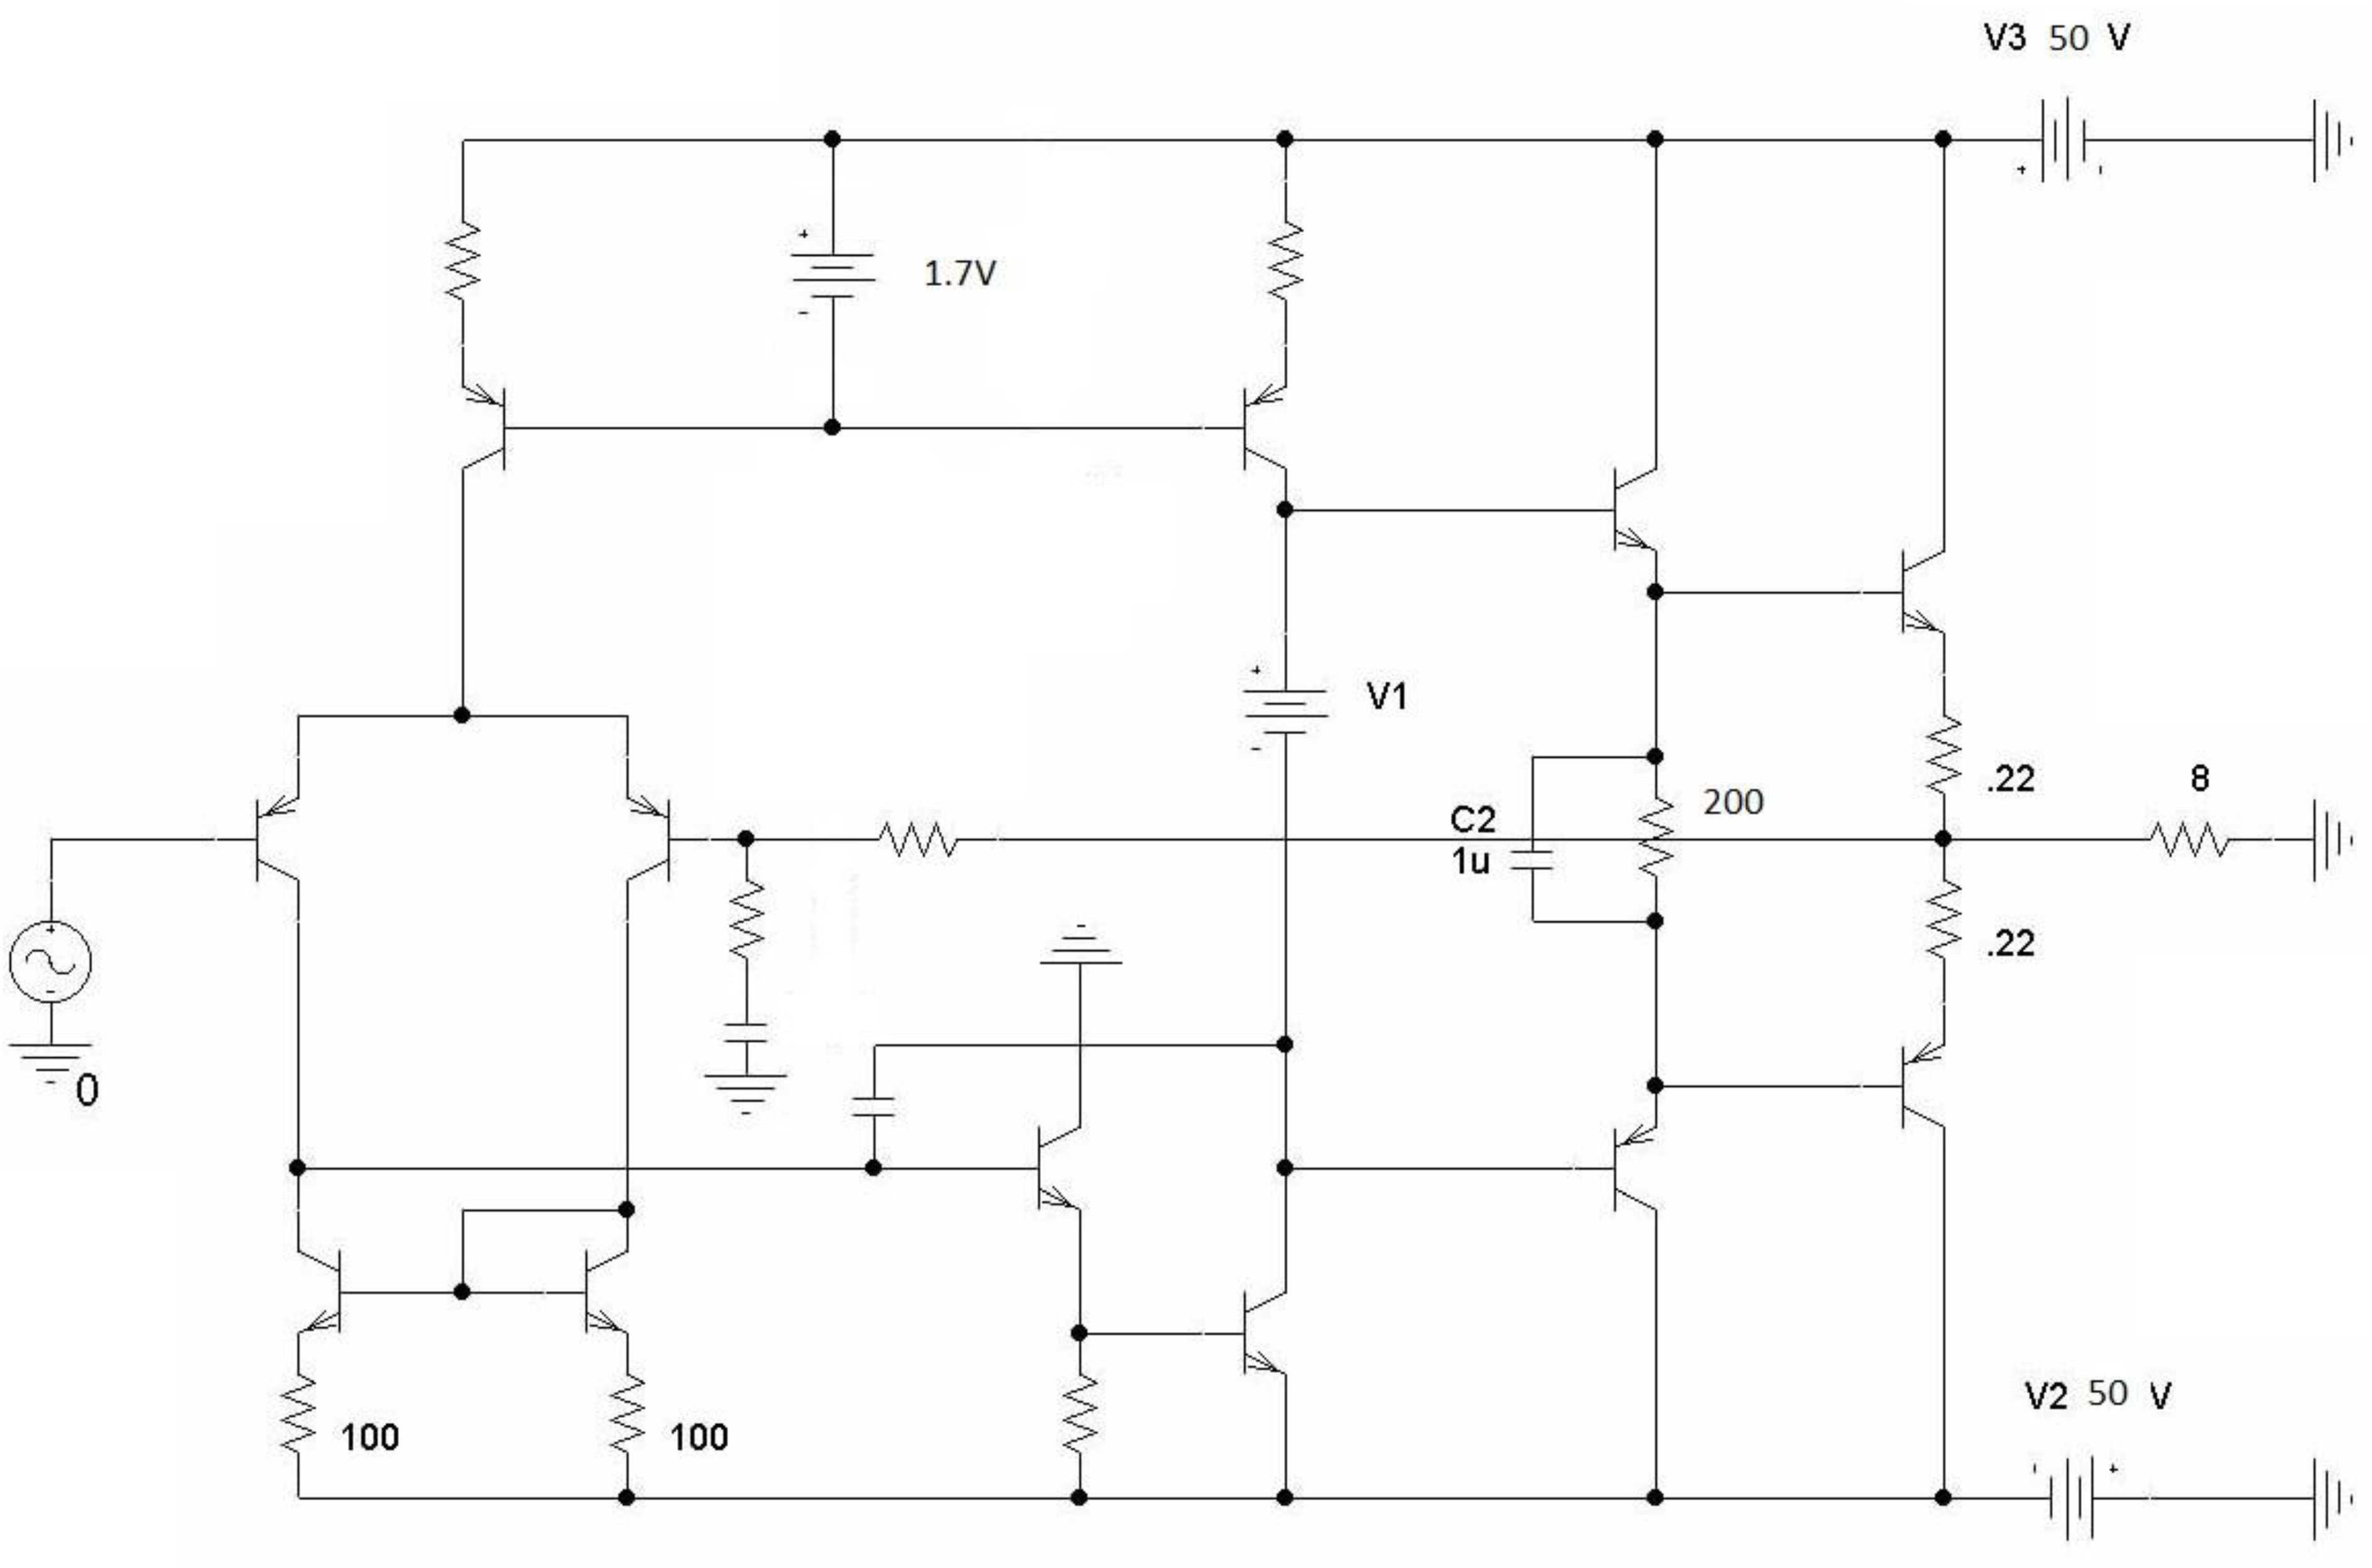
\includegraphics[width=1.0 \textwidth, angle=0]{./img/enunciado/circuito_enunciado.png}
\caption{\label{fig:fig_original_circuit}\footnotesize{Circuito propuesto.}}
\end{center}
\end{figure}


\clearpage

\clearpage
%\\\\\\\\\\\\\\\\\\\\\\\\\\\

%\\\\\\\\\\\\\\\\\\\\\\\\\\\
\section{Punto de reposo}
\resetallcounters

Se hizo inicialmente un cálculo rápido de los valores necesarios para los resistores para lograr el punto Q requerido, luego se refinaron por simulación estos valores, para finalmente llevar a valores comerciales de la serie \textbf{E24} (5 \%) o \textbf{E96} (1 \%), figura~\figref{fig:fig_q_point}. Se utilizaron los de la serie al 1 \% para aquellos resistores que deben estar apareados (espejo de corriente) y para aquellos resistores que fijan la polarización o forman parte de la red de realimentación, en este último caso, también deberían utilizarse resistores de film de óxido metálico, por ser los resistores con mayor estabilidad térmica. En el cuadro~\tableref{table:table_resistors} se muestran los resistores seleccionados y su tipo, y en el cuadro~\tableref{table:table_qpoint} se resumen los valores de polarización finalmente obtenidos.


\begin{figure}[H] %htb
\begin{center}
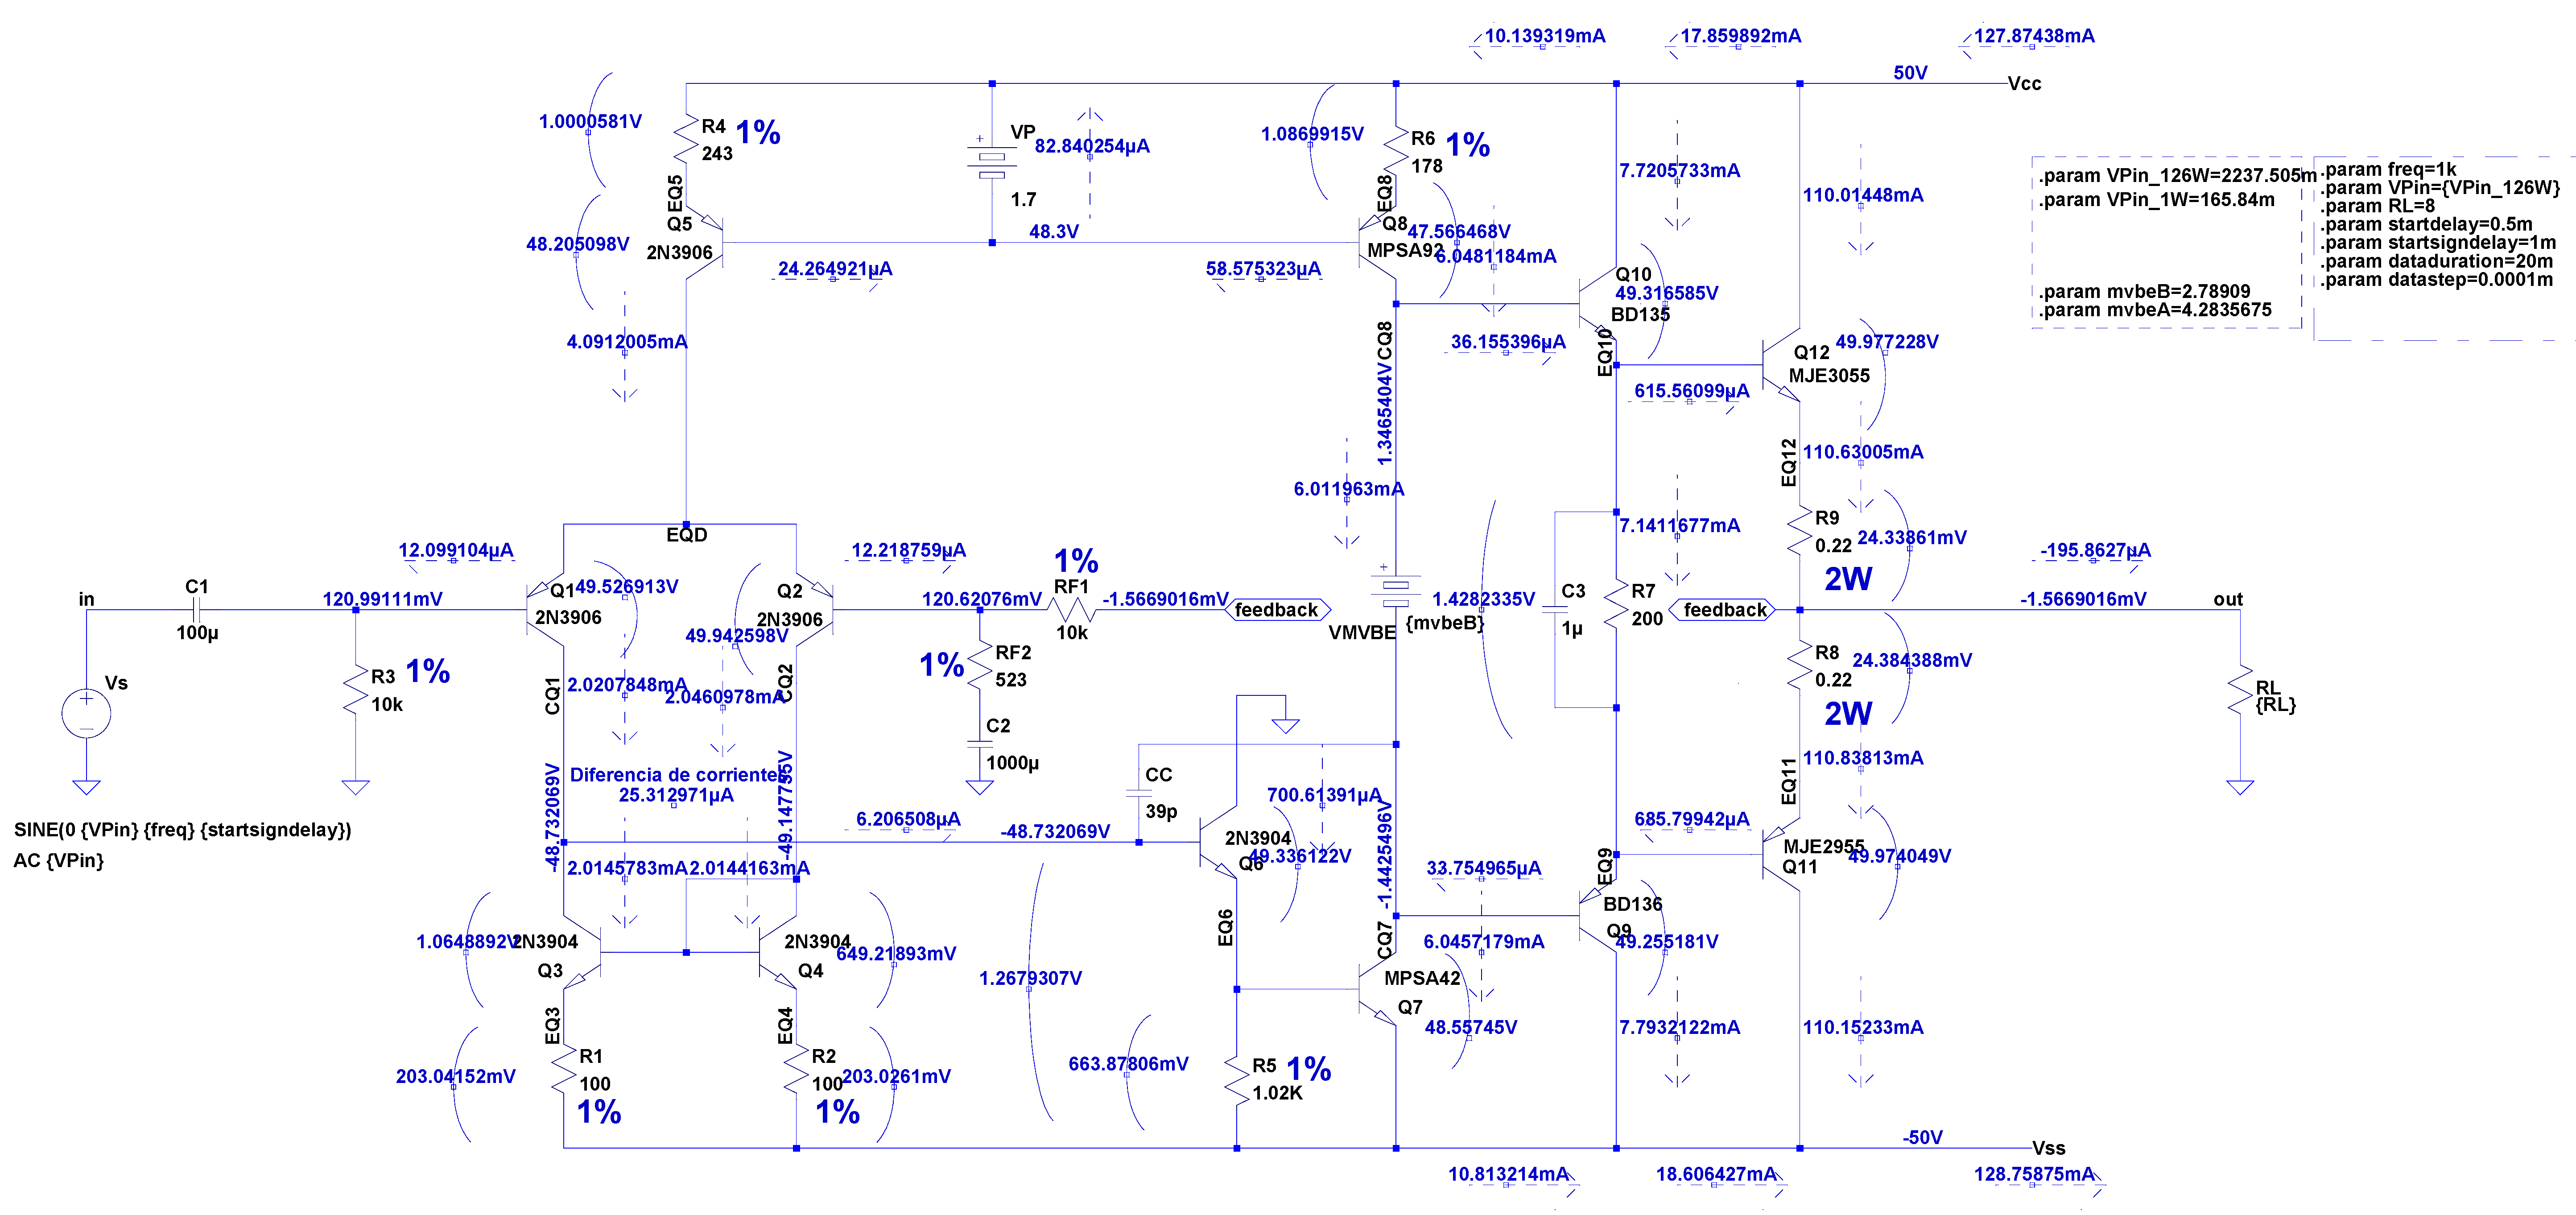
\includegraphics[width=1.1 \textwidth, angle=0]{./img/qpoint/amplifier_qpoint.png}
\caption{\label{fig:fig_q_point}\footnotesize{Punto de reposo.}}
\end{center}
\end{figure}

\clearpage



%% \noindent
%% \begin{center}
 
%%\begin{spacing}{1}  
\begin{table}[H]  %%\centering

    \setlength\arrayrulewidth{1.5pt}
    \arrayrulecolor{white}
    \def\clinecolor{\hhline{|>{\arrayrulecolor{white}}-%
    >{\arrayrulecolor{white}}|-|-|-|-|-|-|-|-|-|-|-|-|}}
\resizebox{0.7 \textwidth}{!}{% 
       
\begin{tabularx}{1 \textwidth}%
    {|
    >{\columncolor{white} \centering\arraybackslash}m{0.15\textwidth}
     |
    >{\columncolor{white} \centering\arraybackslash}m{0.09\textwidth}
     |
    >{\columncolor{white} \centering\arraybackslash}m{0.09\textwidth}
     |
    >{\columncolor{white} \centering\arraybackslash}m{0.09\textwidth}
     |
    >{\columncolor{white} \centering\arraybackslash}m{0.09\textwidth}
     |
    >{\columncolor{white} \centering\arraybackslash}m{0.09\textwidth} 
     |
    >{\columncolor{white} \centering\arraybackslash}m{0.09\textwidth}  
     |
    >{\columncolor{white} \centering\arraybackslash}m{0.09\textwidth}  
     |
    >{\columncolor{white} \centering\arraybackslash}m{0.09\textwidth} 
     |
    >{\columncolor{white} \centering\arraybackslash}m{0.09\textwidth}  
     |
    >{\columncolor{white} \centering\arraybackslash}m{0.09\textwidth} 
     |
    >{\columncolor{white} \centering\arraybackslash}m{0.09\textwidth} 
     |
    }
    \rowcolor{HeadersColor} \cellcolor{white} \thead{}  & \thead{R1} & \thead{R2} & \thead{R3} & \thead{R4} & \thead{R5} & \thead{R6} & \thead{R7} & \thead{R8} & \thead{R9} & \thead{RF1} & \thead{RF2} \\  
    \hhline{|-|-|-|-|-|-|-|-|-|-|-|-|}
    \rowcolor{Butter!20} \cellcolor{Butter!40} $R$ [$\si[per-mode=symbol]{\ohm}$] & \num{100} & \num{100} & \num{10e3} & \num{243} & \num{1.02e3} & \num{178} & \num{200} &  \num{.22} & \num{0.22} & \num{10e3} & \num{523}  \\
    \hhline{|-|-|-|-|-|-|-|-|-|-|-|-|}
    \rowcolor{gray!20} \cellcolor{gray!40} $Tolerancia$ [$\si[per-mode=symbol]{\percent}$] & \num{1} & \num{1} & \num{1} & \num{1} & \num{1} & \num{1} & \num{5} &  \num{5} & \num{5} & \num{1} & \num{1} \\
    \hhline{|-|-|-|-|-|-|-|-|-|-|-|-|}
    \rowcolor{gray!20} \cellcolor{gray!40} $Potencia$ [$\si[per-mode=symbol]{\watt}$] & $\frac{1}{8}$ & $\frac{1}{8}$ & $\frac{1}{8}$ & $\frac{1}{8}$ & $\frac{1}{8}$ & $\frac{1}{8}$ & $\frac{1}{8}$ &  \num{2} & \num{2} & $\frac{1}{8}$ & $\frac{1}{8}$ \\
    \hhline{|-|-|-|-|-|-|-|-|-|-|-|-|}    
    \rowcolor{gray!20} \cellcolor{gray!40} TIPO & Metal Film & Metal Film & Metal Film & Metal Film & Metal Film & Metal Film & Carbon Film & Wired & Wired & Metal Oxide Film & Metal Oxide Film \\
    \end{tabularx}}
	\caption{\footnotesize{Resistores seleccionados.}}
	\label{table:table_resistors}
\end{table}
%%\end{spacing}

%% \end{center}




%% \noindent
%% \begin{center}
 
%%\begin{spacing}{1}  
\begin{table}[H]  %%\centering

    \setlength\arrayrulewidth{1.5pt}
    \arrayrulecolor{white}
    \def\clinecolor{\hhline{|>{\arrayrulecolor{white}}-%
    >{\arrayrulecolor{white}}|-|-|-|-|-|-|-|-|-|-|-|-|-|}}
\resizebox{0.66 \textwidth}{!}{% 
       
\begin{tabularx}{1 \textwidth}%
    {|
    >{\columncolor{white} \centering\arraybackslash}m{0.13\textwidth}
     |
    >{\columncolor{white} \centering\arraybackslash}m{0.09\textwidth}
     |
    >{\columncolor{white} \centering\arraybackslash}m{0.09\textwidth}
     |
    >{\columncolor{white} \centering\arraybackslash}m{0.09\textwidth}
     |
    >{\columncolor{white} \centering\arraybackslash}m{0.09\textwidth}
     |
    >{\columncolor{white} \centering\arraybackslash}m{0.09\textwidth} 
     |
    >{\columncolor{white} \centering\arraybackslash}m{0.09\textwidth}  
     |
    >{\columncolor{white} \centering\arraybackslash}m{0.09\textwidth}  
     |
    >{\columncolor{white} \centering\arraybackslash}m{0.09\textwidth} 
     |
    >{\columncolor{white} \centering\arraybackslash}m{0.09\textwidth}  
     |
    >{\columncolor{white} \centering\arraybackslash}m{0.09\textwidth} 
     |
    >{\columncolor{white} \centering\arraybackslash}m{0.09\textwidth} 
     |
    >{\columncolor{white} \centering\arraybackslash}m{0.09\textwidth} 
     |
    }
    \rowcolor{HeadersColor} \cellcolor{white} \thead{}  & \thead{Q1} & \thead{Q2} & \thead{Q3} & \thead{Q4} & \thead{Q5} & \thead{Q6} & \thead{Q7} & \thead{Q8} & \thead{Q9} & \thead{Q10} & \thead{Q11} & \thead{Q12} \\
    
    \hhline{|-|-|-|-|-|-|-|-|-|-|-|-|-|}
    \rowcolor{gray!20} \cellcolor{gray!40} MODEL & 2N3906 & 2N3906 & 2N3904 & 2N3904 & 2N3906 & 2N3904 & MPSA42 & MPSA92 & BD136 & BD135 & MJE2955 & MJE3055  \\
    \hhline{|-|-|-|-|-|-|-|-|-|-|-|-|-|}
    \rowcolor{Butter!20} \cellcolor{Butter!40} $I_{C}$ [$\si[per-mode=symbol]{\ampere}$] & \num{2.02e-3} & \num{2.05e-3} & \num{2.01e-3} & \num{2.01e-3} & \num{4.09e-3} & \num{700.61e-6} & \num{6.05e-3} &  \num{6.05e-3} & \num{7.79e-3} & \num{7.72e-3} & \num{110.00e-3} & \num{110.14e-3}  \\
    \hhline{|-|-|-|-|-|-|-|-|-|-|-|-|-|}
    \rowcolor{gray!20} \cellcolor{gray!40} $gm$ [$\si[per-mode=symbol]{\milli\ampere\per\volt}$] & \num{56.00} & \num{56.60} & \num{48.10} & \num{48.10} & \num{111.00} & \num{17.50} & \num{20.40} & \num{22.90} & \num{300} & \num{298.00} & \num{4060.00}  & \num{4170.00} \\
    \hhline{|-|-|-|-|-|-|-|-|-|-|-|-|-|}
    \rowcolor{gray!20} \cellcolor{gray!40} $r_{o}$ [$\si[per-mode=symbol]{\ohm}$] & \num{92.7e+03} & \num{91.7e+03} & \num{462.0e+03} & \num{462.0e+03} & \num{45.3e+03} & \num{1.41e+06} & \num{24.5e+03} & \num{24.3e+03} & \num{18.5e+03} & \num{21.3e+03} & \num{1.36e+03} & \num{903.0}  \\
    \hhline{|-|-|-|-|-|-|-|-|-|-|-|-|-|}
    \rowcolor{gray!20} \cellcolor{gray!40} $\beta [AC]$ & 174 & 174 & 140 & 140 & 170 & 143 & 157 & 108 & 242  & 223 & 162 & 196  \\
    \hhline{|-|-|-|-|-|-|-|-|-|-|-|-|-|}
    \rowcolor{gray!20} \cellcolor{gray!40}  $r_{\pi}$ [$\si[per-mode=symbol]{\ohm}$] & \num{3.10e3} & \num{3.07e3} & \num{2.90e3} & \num{2.90e3} & \num{1.53e3}  & \num{8.17e3}  & \num{772.0} & \num{472.0} & \num{806.0} & \num{748.0} & \num{40.0} & \num{47.0}  \\
    \hhline{|-|-|-|-|-|-|-|-|-|-|-|-|-|}
    \rowcolor{gray!20} \cellcolor{gray!40} $f_{T}$ [$\si[per-mode=symbol]{\mega\hertz}$] & \num{210.00} & \num{211.00} & \num{227.00} & \num{222.00} & \num{247.00} & \num{164.00} & \num{74.90} & \num{81.10} & \num{115.00} & \num{178.00} & \num{6.80} & \num{4.24}  \\         
    \end{tabularx}}
	\caption{\footnotesize{$I_{C_{Q}}$ y elementos del modelo de pequeña señal de los transistores.}}
	\label{table:table_qpoint}
\end{table}
%%\end{spacing}

%% \end{center}

El capacitor $C_{1}$ que se coloca para impedir que continua aplicada al circuito altere la polarización, debería ser un electrolítico de buena calidad, y su valor de $100 \si[per-mode=symbol]{\micro\farad}$  se seleccionó para cumplir con la misma frecuencia de corte inferior que para $C_{1}$. \\

El capacitor $C_{2}$ de $1000 \si[per-mode=symbol]{\micro\farad}$ se seleccionó para tener una frecuencia de corte inferior de como máximo $20 \si[per-mode=symbol]{\hertz}$, y debería ser un capacitor electrolítico de buena calidad, de bajo ESR y no polarizado. \\

El capacitor $C_{C}$, de $39 \si[per-mode=symbol]{\pico\farad}$, que se coloca para realizar la compensación de Miller, debería ser un capacitor de poliestireno o polietileno.



\clearpage
%\\\\\\\\\\\\\\\\\\\\\\\\\\\

%\\\\\\\\\\\\\\\\\\\\\\\\\\\
\section{Capacitores utilizados en el circuito}
\resetallcounters

El capacitor $C_{1}$ que se coloca para impedir que continua aplicada al circuito por la fuente de la señal de audio, o una etapa previa, altere la polarización, debería ser un capacitor electrolítico no polarizado, y su valor de $100 \si[per-mode=symbol]{\micro\farad}$ se seleccionó para cumplir con una frecuencia de corte inferior de como máximo $20 \si[per-mode=symbol]{\hertz}$, y no influir significativamente en el THD a bajas frecuencias. Con un valor de $47 \si[per-mode=symbol]{\micro\farad}$ sería suficiente para cumplir con la frecuencia de corte inferior, pero su influencia sobre el THD se hace apreciable incluso a $1 \si[per-mode=symbol]{\kilo\hertz}$ \\

El capacitor $C_{2}$ de $1000 \si[per-mode=symbol]{\micro\farad}$ se seleccionó para que no tenga efecto apreciable sobre el THD, especialmente a bajas frecuencias, y debería ser un capacitor electrolítico de buena calidad, de bajo ESR y no polarizado. La calidad de este capacitor es crítica por hallarse en la red de realimentación, influyendo directamente en la calidad y estabilidad del amplificador. En un circuito mas completo deberían agregarse diodos que protejan este capacitor de un valor de tensión que podría aparecer a la salida, en caso de saturación, que supere su máxima tensión de trabajo. \\

El capacitor $C_{C}$, de $39 \si[per-mode=symbol]{\pico\farad}$, ver sección~\sectref{sect:compensation}, que se coloca para realizar la compensación de Miller, debería ser un capacitor de poliestireno o poliéster.


\vfill




\clearpage
%\\\\\\\\\\\\\\\\\\\\\\\\\\\

%\\\\\\\\\\\\\\\\\\\\\\\\\\\
\section{Análisis cualitativo}
\resetallcounters

\normalfont

La topología del circuito corresponde a la de un típico amplificador de potencia de tres etapas realimentado, la tensión de salida es muestreada y sumada a la entrada, formando un lazo de realimentación \textbf{serie-paralelo}, estabilizando la tensión de salida. \\

En el circuito se pueden diferenciar claramente las tres etapas, las mismas son:


\begin{itemize}
\item Amplificador diferencial con caga activa (espejo de corriente con degeneración de emisor): realiza la suma (resta) de la señal de entrada con la señal realimentada y provee amplificación.
\item VAS: Formado por un seguidor polarizado con la tensión de colector de la primera etapa, que provee adaptación de impedancia entre la primera etapa (permitiendo que el par diferencial provea alta ganancia, aprovechando su carga activa) y un emisor común con carga activa (fuente de corriente simple con degeneración de emisor), que provee la ganancia. Es en esta etapa que se realiza la compensación de Miller con un capacitor.
\item Etapa de salida push-pull formada con Darlingtons complementarios.
\end{itemize}

Con un muy rápido análisis aproximado por inspección, se obtiene una ganancia para el amplificador de tres etapas de alrededor de $130 \si[per-mode=symbol]{\decibel}$, obteniéndose con este valor para la ganancia de lazo, alrededor de $110 \si[per-mode=symbol]{\decibel}$, este valor se ajusta muy bien para un análisis aproximado, con el valor obtenido por simulación a frecuencias medias.







\clearpage
%\\\\\\\\\\\\\\\\\\\\\\\\\\\

%\\\\\\\\\\\\\\\\\\\\\\\\\\\
\section{Compensación}
\resetallcounters

\label{sect:compensation}

Para realizar la compensación de Miller del amplificador, y determinar el valor del capacitor, es necesario relevar la ganancia de lazo con la frecuencia. Teóricamente para realizar una compensación por polo dominante con un margen de fase de $45 \si[per-mode=symbol]{\degree}$, debería colocarse el polo, de tal forma de que la ganancia de lazo sea de exactamente $0 \si[per-mode=symbol]{\decibel}$, donde se encuentre el primer polo natural del circuito. La técnica usada prácticamente es observar en forma aproximada donde se localiza este punto y con un valor aproximado de la resistencia a frecuencias medias \quotemarks{vista} por el capacitor de Miller, determinada por inspección, tener una primera aproximación de la frecuencia del polo, usando el $\tau_{RC}$ calculado aproximadamente, luego el valor se refina por prueba y error, para finalmente llevar el valor óptimo a un valor comercial. El circuito utilizado para relevar la ganancia de lazo se puede observar en la figura~\figref{fig:fig_circuit_compensation}, en el mismo se introduce la señal de prueba a través de la entrada inversora del amplificador diferencial con un capacitor de acople de alto valor, luego de haber pasivado la señal de entrada, se introduce un resistor de \quotemarks{separación}, que permite observar la señal en la salida del amplificador, luego de haber pasado por la red de realimentación y el amplificador, obteniéndose de esta forma la ganancia de lazo. Se pretende mantener el punto de reposo inalterado, para lograr esto, se altera también el resistor colocado en la otra entrada del amplificador diferencial, de manera de compensar el offset que se produce por la caída provocada por las corrientes de base de los transistores del par diferencial.\\

El valor determinado aproximadamente, está en el orden de las decenas de $\si[per-mode=symbol]{\pico\farad}$, por lo tanto se partió de un valor de $100 \si[per-mode=symbol]{\pico\farad}$, el cual se fue bajando hasta lograr la compensación buscada. \\

El valor comercial seleccionado finalmente para el capacitor de compensación es de  $39 \si[per-mode=symbol]{\pico\farad}$. En la figura~\figref{fig:fig_loop_gain} se puede observar el gráfico de la ganancia de lazo en magnitud y fase resultante, el mismo se realizó en \textbf{MATLAB} con datos exportados desde \textbf{LTSPICE}, para mayor claridad. \\

Algo importante a observar, es que se observa un par de polos complejos conjugados alrededor de los $25 \si[per-mode=symbol]{\mega\hertz}$, este par de polos introducen un giro de fase extra de $90 \si[per-mode=symbol]{\degree}$, además del sobre-pico en la ganancia, llevando al amplificador mas cerca de la inestabilidad a esta frecuencia. Es posible que en este caso, a pesar de haberse logrado una compensación correcta a $45 \si[per-mode=symbol]{\degree}$, sea conveniente llevar ese margen a un valor un poco mayor. Estos polos que se observan parecen ser introducidos por los transistores usados en el VAS, \textbf{MPSA42} y \textbf{MPSA92}, no se observa al reemplazar los mismos con otros transistores, podría ser una peculiaridad de los transistores o de los modelos (proveídos por el fabricante).

\clearpage

\begin{figure}[H] %htb
\begin{center}
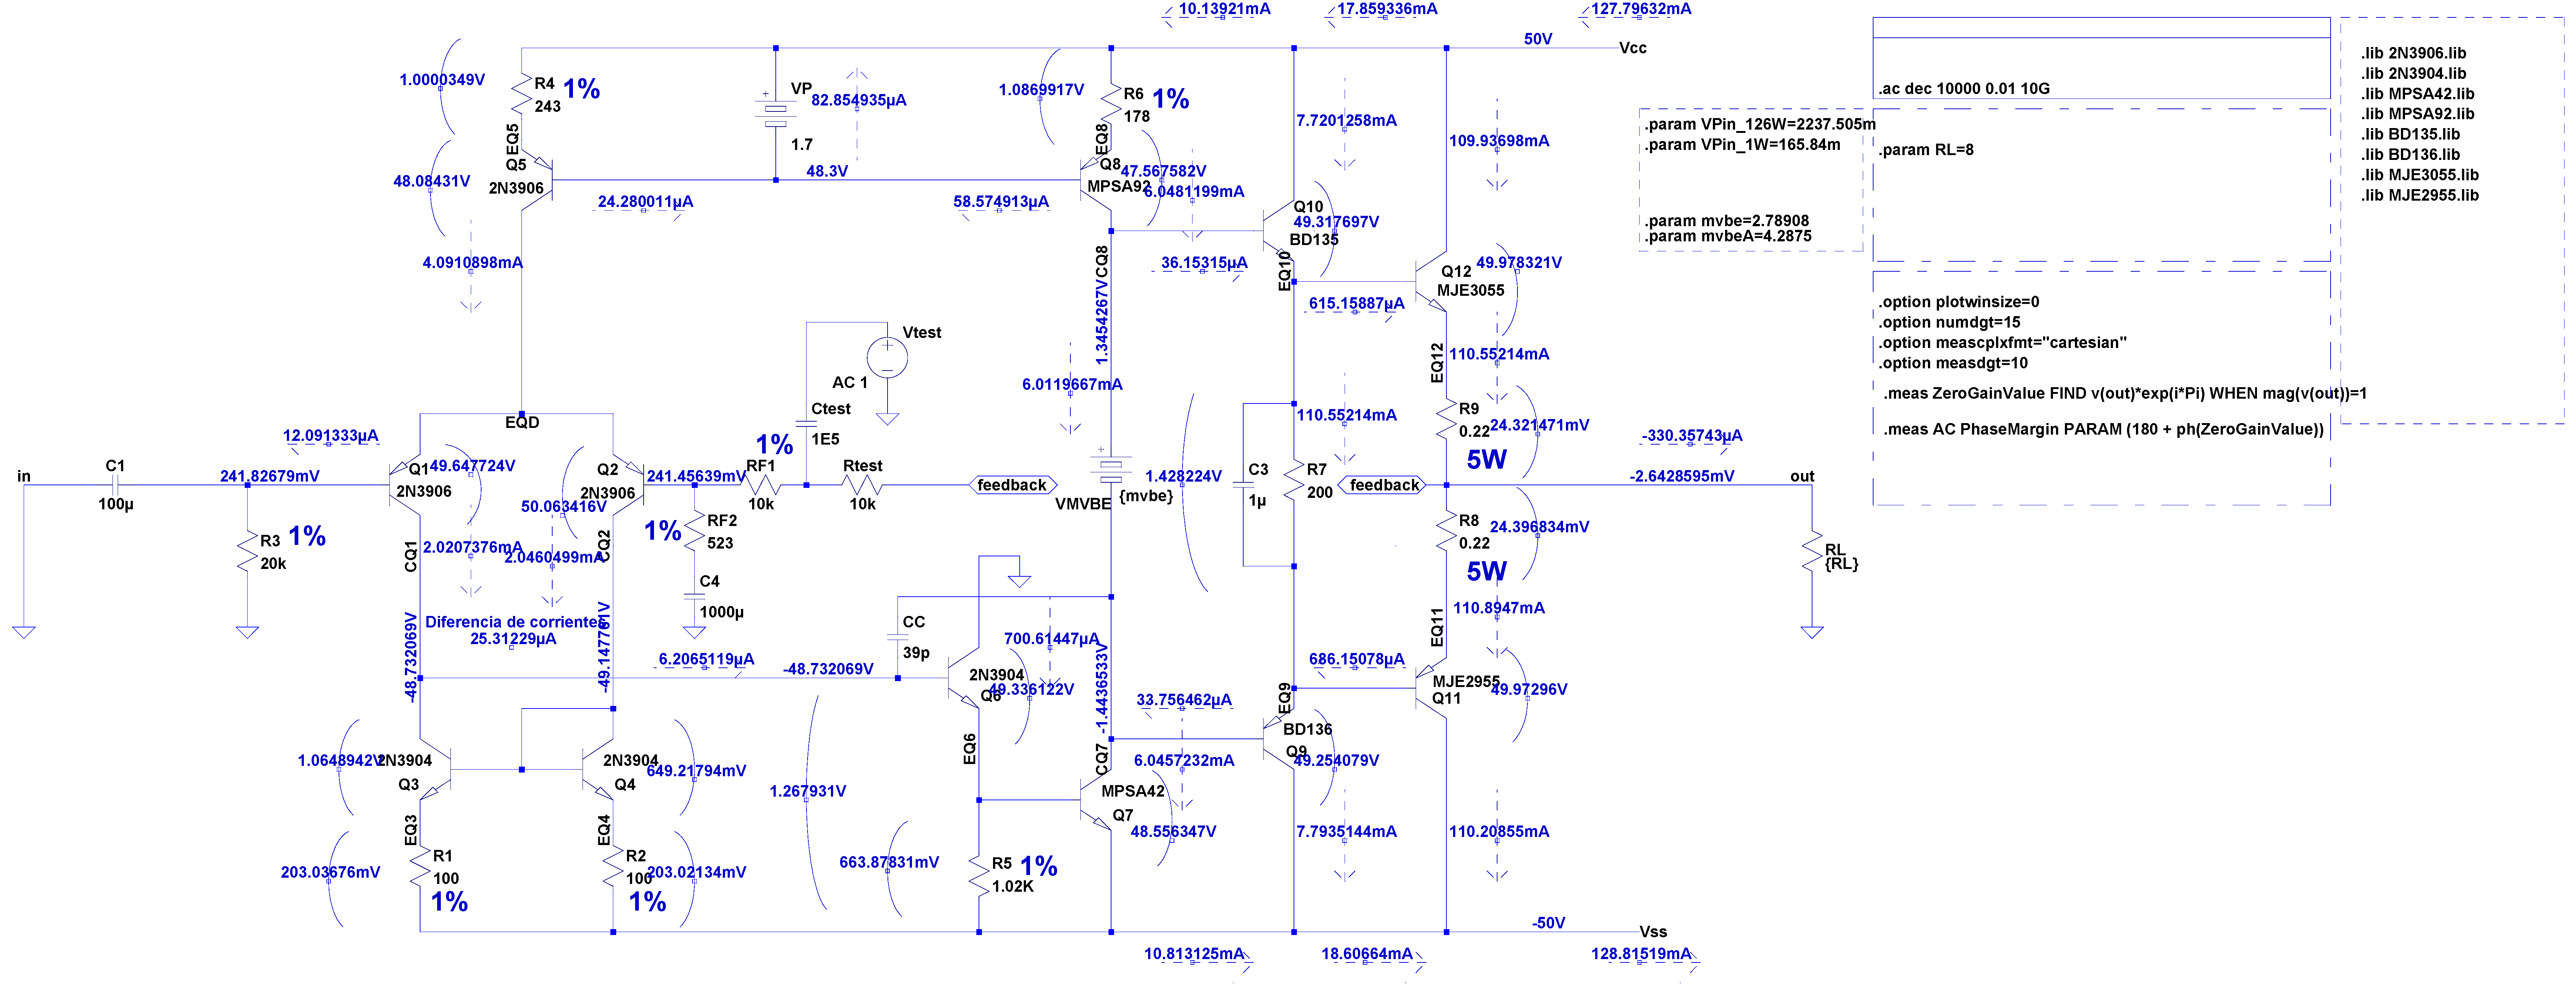
\includegraphics[width=0.93 \textheight, angle=90]{./img/circuits/amplifier_LOOP.png}
\caption{\label{fig:fig_circuit_compensation}\footnotesize{Circuito usado para determinar la ganancia de lazo.}}
\end{center}
\end{figure}

\clearpage

\begin{figure}[H] %htb
\begin{center}
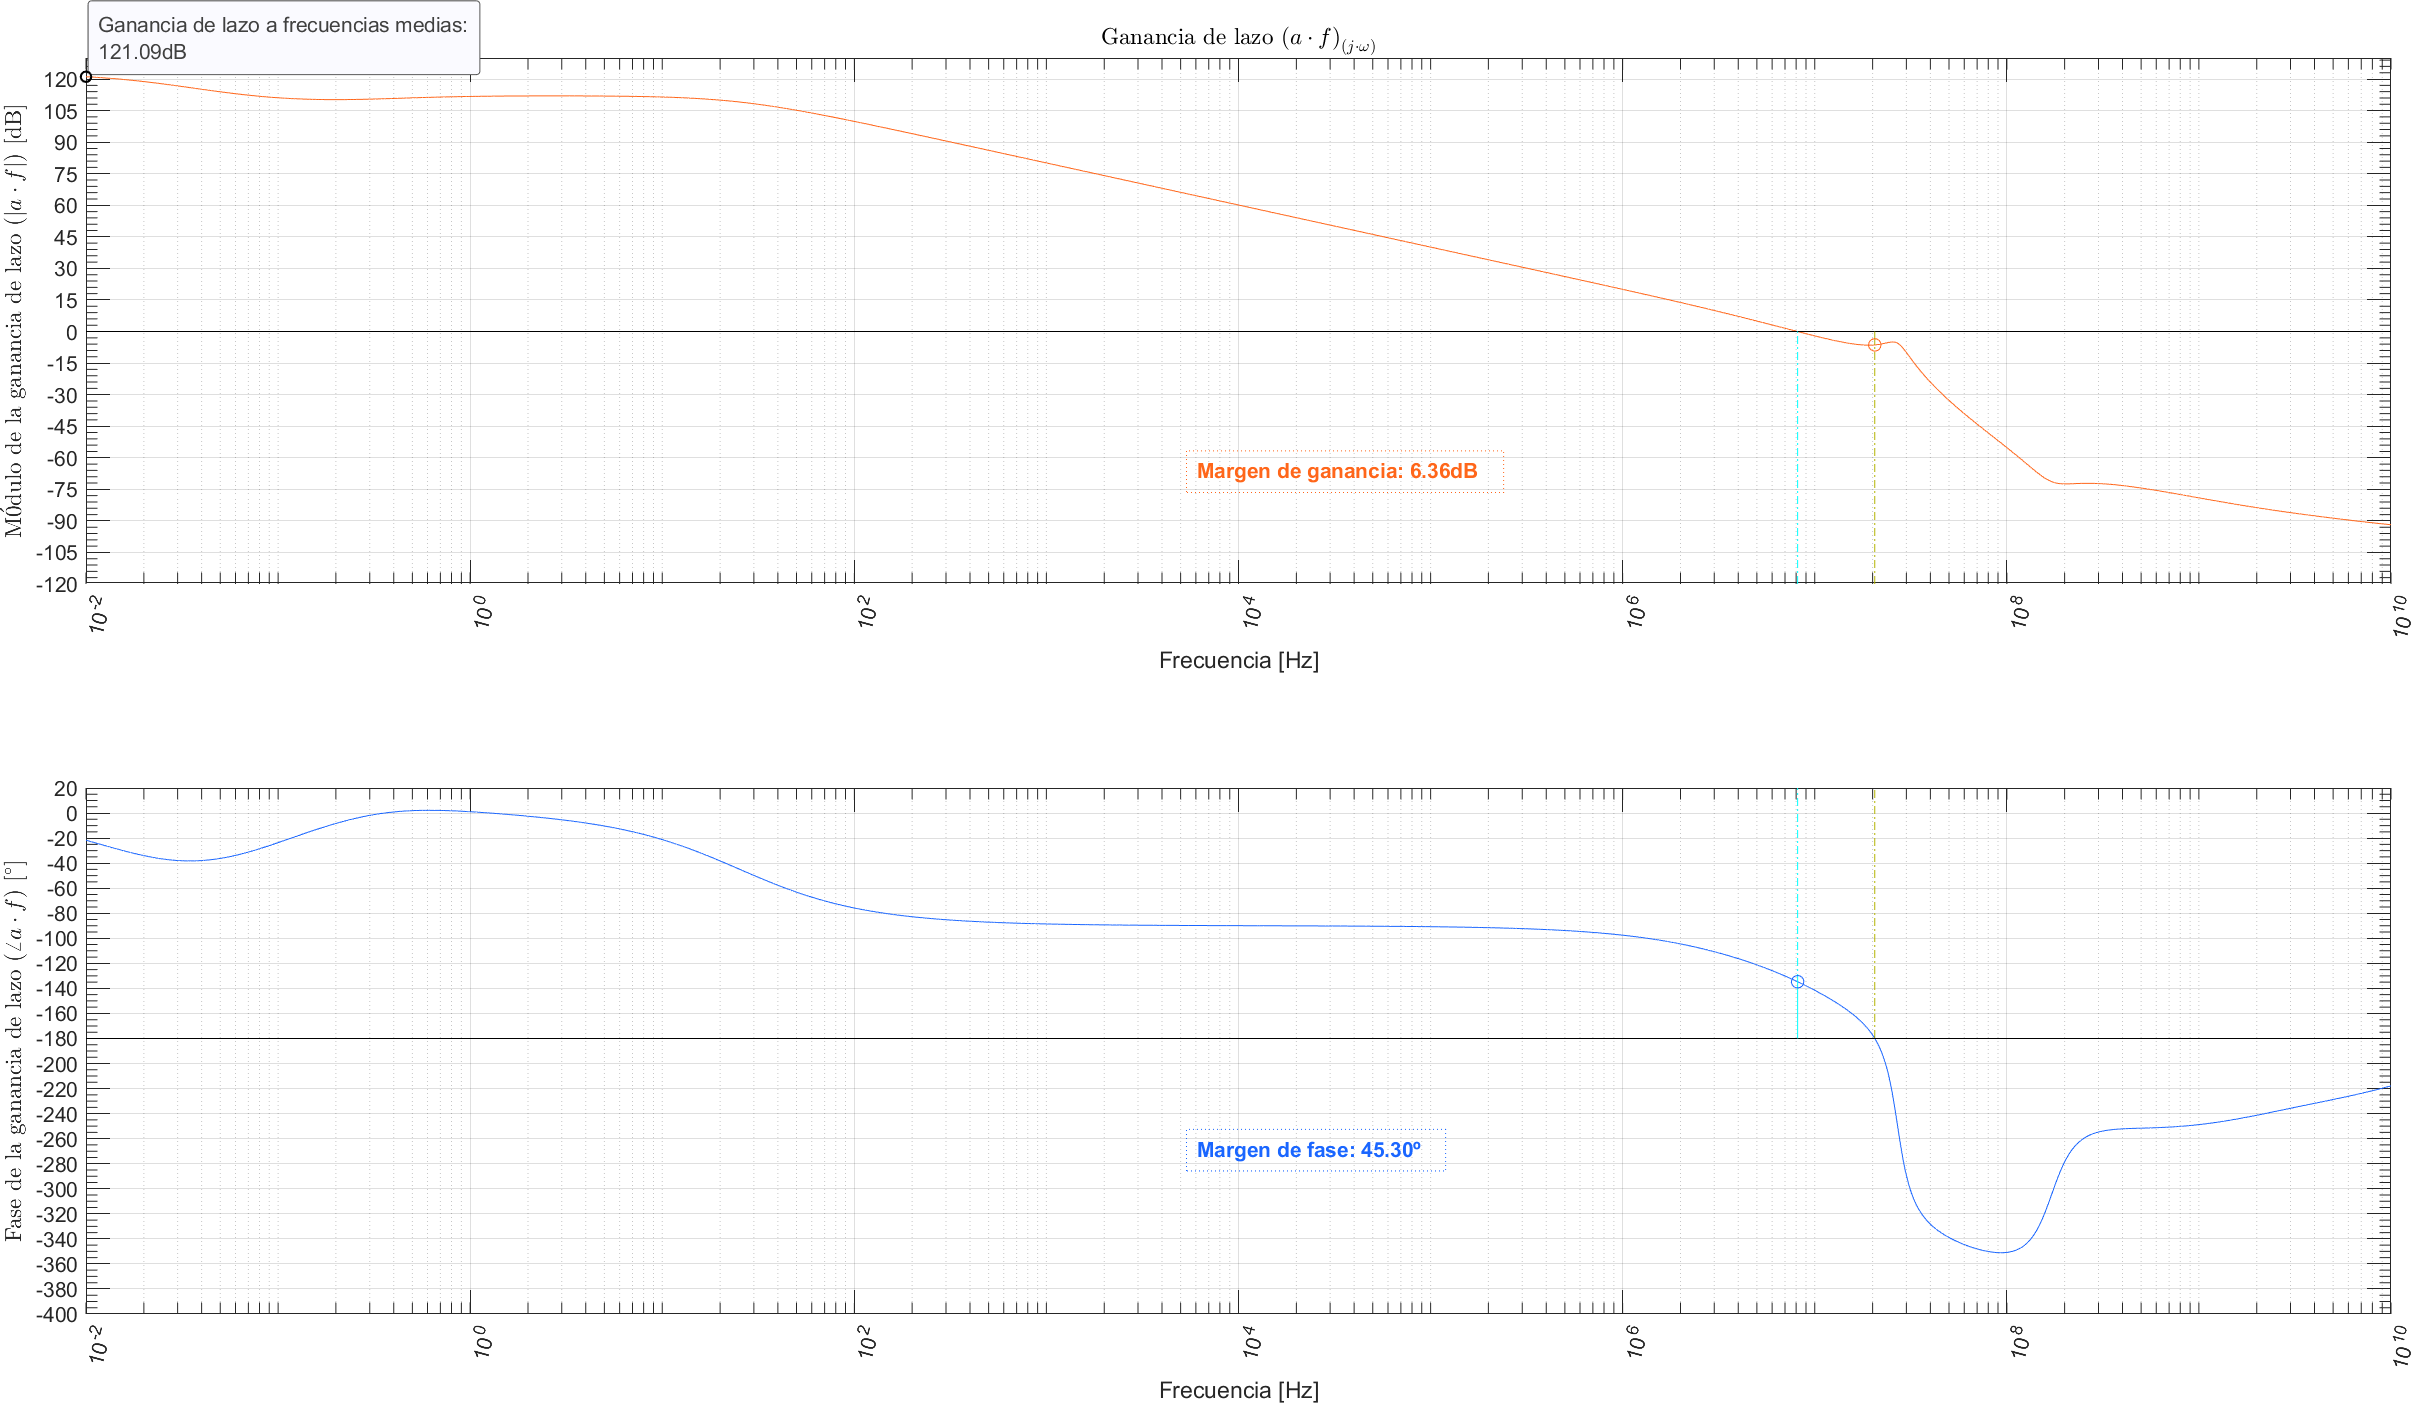
\includegraphics[width=0.93 \textheight, angle=90]{./img/simulaciones/Loop/gain_loop.png}
\caption{\label{fig:fig_loop_gain}\footnotesize{Ganancia de lazo en función de la frecuencia, indicando los márgenes obtenidos.}}
\end{center}
\end{figure}

\clearpage
\clearpage
%\\\\\\\\\\\\\\\\\\\\\\\\\\\


%\\\\\\\\\\\\\\\\\\\\\\\\\\\
\section{Evaluación de la distorsión armónica}
\resetallcounters

Todos los cálculos de la distorsión armónica total (\textbf{THD}), se realizaron evaluando la \textbf{FFT} de la señal de salida, para los primeros \num{10} armónicos de la señal, usando los datos exportados en \textbf{MATLAB}, sin embargo el valor obtenido es exactamente el mismo que proporciona \textbf{LTSPICE}, usando el comando  \mbox{\textbf{\quotemarks{.fourier {freq} 10 4 V(out)}}}, el cual limita el análisis a 10 armónicos, y tomando una cantidad entera de ciclos al final de la señal, para asegurar que el cálculo sea correcto, también se usó un comando para maximizar la precisión numérica, \mbox{\textbf{\quotemarks{.option numdgt=15}}} y se deshabilitó la compresión de datos como se recomienda en el manual, con el comando \mbox{\textbf{\quotemarks{.option plotwinsize=0}}}. Al menos en su última versión el programa parece hacer correctamente esta medición. 

\subsection{Amplificador funcionando en clase \textbf{A} }

Para lograr que el amplificador opere en este modo, simplemente se aumentó la corriente de reposo de la etapa de salida, ajustando el \quotemarks{multiplicador de $V_{BE}$}, hasta lograr que la corriente alcance en cada rama la mitad del valor eficaz, de la corriente que circula por la carga a máxima potencia, aunque esta definición de clase \textbf{A}, para una etapa push-pull, no parece ser la única que se adopta. \\
En nuestro caso a máxima potencia se tiene:

\begin{equation*}
P_{Max} = \frac{{45 \si[per-mode=symbol]{\volt}}^2}{2 \cdot 8\si[per-mode=symbol]{\ohm}} \approx 126.56 \si[per-mode=symbol]{\watt}
\end{equation*}


\begin{equation*}
I_{L_{Max}} = \frac{45 \si[per-mode=symbol]{\volt}}{8\si[per-mode=symbol]{\ohm}} = 5.625 \si[per-mode=symbol]{\ampere} \longrightarrow I_{L_{Eff}} \approx 3.9774 \si[per-mode=symbol]{\ampere}
\end{equation*}


Llevar a clase \textbf{A}, entonces según la interpretación aceptada, es llevar la corriente de polarización de cada uno de los transistores de salida a un valor correspondiente al valor pico asociado a la mitad del valor eficaz calculado anteriormente, tenemos entonces:

\begin{equation*}
\frac{I_{L_{Eff}}}{2} = 1.9887 \si[per-mode=symbol]{\ampere} \longrightarrow I_{C_{Q_{output}}} \approx \sqrt{2} \cdot 1.9887 \si[per-mode=symbol]{\ampere} = 2.8125 \si[per-mode=symbol]{\ampere}
\end{equation*}


\subsection{Simulación del \textbf{THD} con compensación a $45.30 \si[per-mode=symbol]{\degree}$ }

A continuación se obtuvieron los valores correspondientes para el circuito operando en clase \textbf{A}, 
En la tabla~\tableref{table:table_THD_vs_freq_and_compensation} se resumen los valores para el amplificador funcionando en clase \textbf{B} y en clase clase \textbf{A}, con el amplificador compensado a $45.30 \si[per-mode=symbol]{\degree}$.


%% \noindent
%% \begin{center}
 
%%\begin{spacing}{1}  
\begin{table}[H]  %%\centering

    \setlength\arrayrulewidth{1.5pt}
    \arrayrulecolor{white}
    \def\clinecolor{\hhline{|>{\arrayrulecolor{white}}-%
    >{\arrayrulecolor{white}}|-|-|-|}}
\resizebox{0.85 \textwidth}{!}{% 
       
\begin{tabularx}{1 \textwidth}%
    {|
    >{\columncolor{white} \centering\arraybackslash}m{0.33\textwidth}
     |
    >{\columncolor{white} \centering\arraybackslash}m{0.33\textwidth}
     |
    >{\columncolor{white} \centering\arraybackslash}m{0.33\textwidth}
     |
    }
    \rowcolor{HeadersColor}  \cellcolor{white} \thead{}  & \thead{$1 \si[per-mode=symbol]{\kilo\hertz}$} & \thead{$10 \si[per-mode=symbol]{\kilo\hertz}$} \\  
    \hhline{|-|-|-|}
    \rowcolor{gray!20} \cellcolor{gray!40} THD [clase \textbf{B}] & $0.000076 \si[per-mode=symbol]{\percent}$ & $0.000151 \si[per-mode=symbol]{\percent}$ \\
    \hhline{|-|-|-|}
    \rowcolor{gray!20} \cellcolor{gray!40} THD [clase \textbf{A}] & $0.000065 \si[per-mode=symbol]{\percent}$ & $0.000118 \si[per-mode=symbol]{\percent}$ \\
    \end{tabularx}}
	\caption{\footnotesize{THD obtenido a $1 \si[per-mode=symbol]{\kilo\hertz}$ y $10 \si[per-mode=symbol]{\kilo\hertz}$ para modo de operación en clase \textbf{B} y clase \textbf{A}, compensado a $45.30 \si[per-mode=symbol]{\degree}$.}}
	\label{table:table_THD_vs_freq_and_compensation}
\end{table}
%%\end{spacing}

%% \end{center}


\subsection{Simulación del \textbf{THD} con compensación a $81.76 \si[per-mode=symbol]{\degree}$ }


A continuación se repitieron todas las simulaciones para determinar el \textbf{THD} del amplificador en las mismas condiciones de antes, solo que ahora se llevó el capacitor de compensación a un valor un orden magnitud mayor, $390 \si[per-mode=symbol]{\pico\farad}$. En la figura~\figref{fig:fig_loop_gain_2} se puede observar el resultado para los márgenes con la nueva compensación. \\

En la tabla~\tableref{table:table_THD_vs_freq_and_compensation_2} se resumen los valores para el amplificador funcionando en clase \textbf{B} y en clase clase \textbf{A}, con el amplificador con la nueva compensación a $81.76 \si[per-mode=symbol]{\degree}$. \\



%% \noindent
%% \begin{center}
 
%%\begin{spacing}{1}  
\begin{table}[H]  %%\centering

    \setlength\arrayrulewidth{1.5pt}
    \arrayrulecolor{white}
    \def\clinecolor{\hhline{|>{\arrayrulecolor{white}}-%
    >{\arrayrulecolor{white}}|-|-|-|}}
\resizebox{0.85 \textwidth}{!}{% 
       
\begin{tabularx}{1 \textwidth}%
    {|
    >{\columncolor{white} \centering\arraybackslash}m{0.33\textwidth}
     |
    >{\columncolor{white} \centering\arraybackslash}m{0.33\textwidth}
     |
    >{\columncolor{white} \centering\arraybackslash}m{0.33\textwidth}
     |
    }
    \rowcolor{HeadersColor}  \cellcolor{white} \thead{}  & \thead{$1 \si[per-mode=symbol]{\kilo\hertz}$} & \thead{$10 \si[per-mode=symbol]{\kilo\hertz}$} \\  
    \hhline{|-|-|-|}
    \rowcolor{gray!20} \cellcolor{gray!40} THD [clase \textbf{B}] & $0.000139 \si[per-mode=symbol]{\percent}$ & $0.007023 \si[per-mode=symbol]{\percent}$ \\
    \hhline{|-|-|-|}
    \rowcolor{gray!20} \cellcolor{gray!40} THD [clase \textbf{A}] & $0.000116 \si[per-mode=symbol]{\percent}$ & $0.005266 \si[per-mode=symbol]{\percent}$ \\
    \end{tabularx}}
	\caption{\footnotesize{THD obtenido a $1 \si[per-mode=symbol]{\kilo\hertz}$ y $10 \si[per-mode=symbol]{\kilo\hertz}$ para modo de operación en clase \textbf{B} y clase \textbf{A}, compensado a $81.76 \si[per-mode=symbol]{\degree}$.}}
	\label{table:table_THD_vs_freq_and_compensation_2}
\end{table}
%%\end{spacing}

%% \end{center}


\vspace*{\fill}


\clearpage

\begin{figure}[H] %htb
\begin{center}
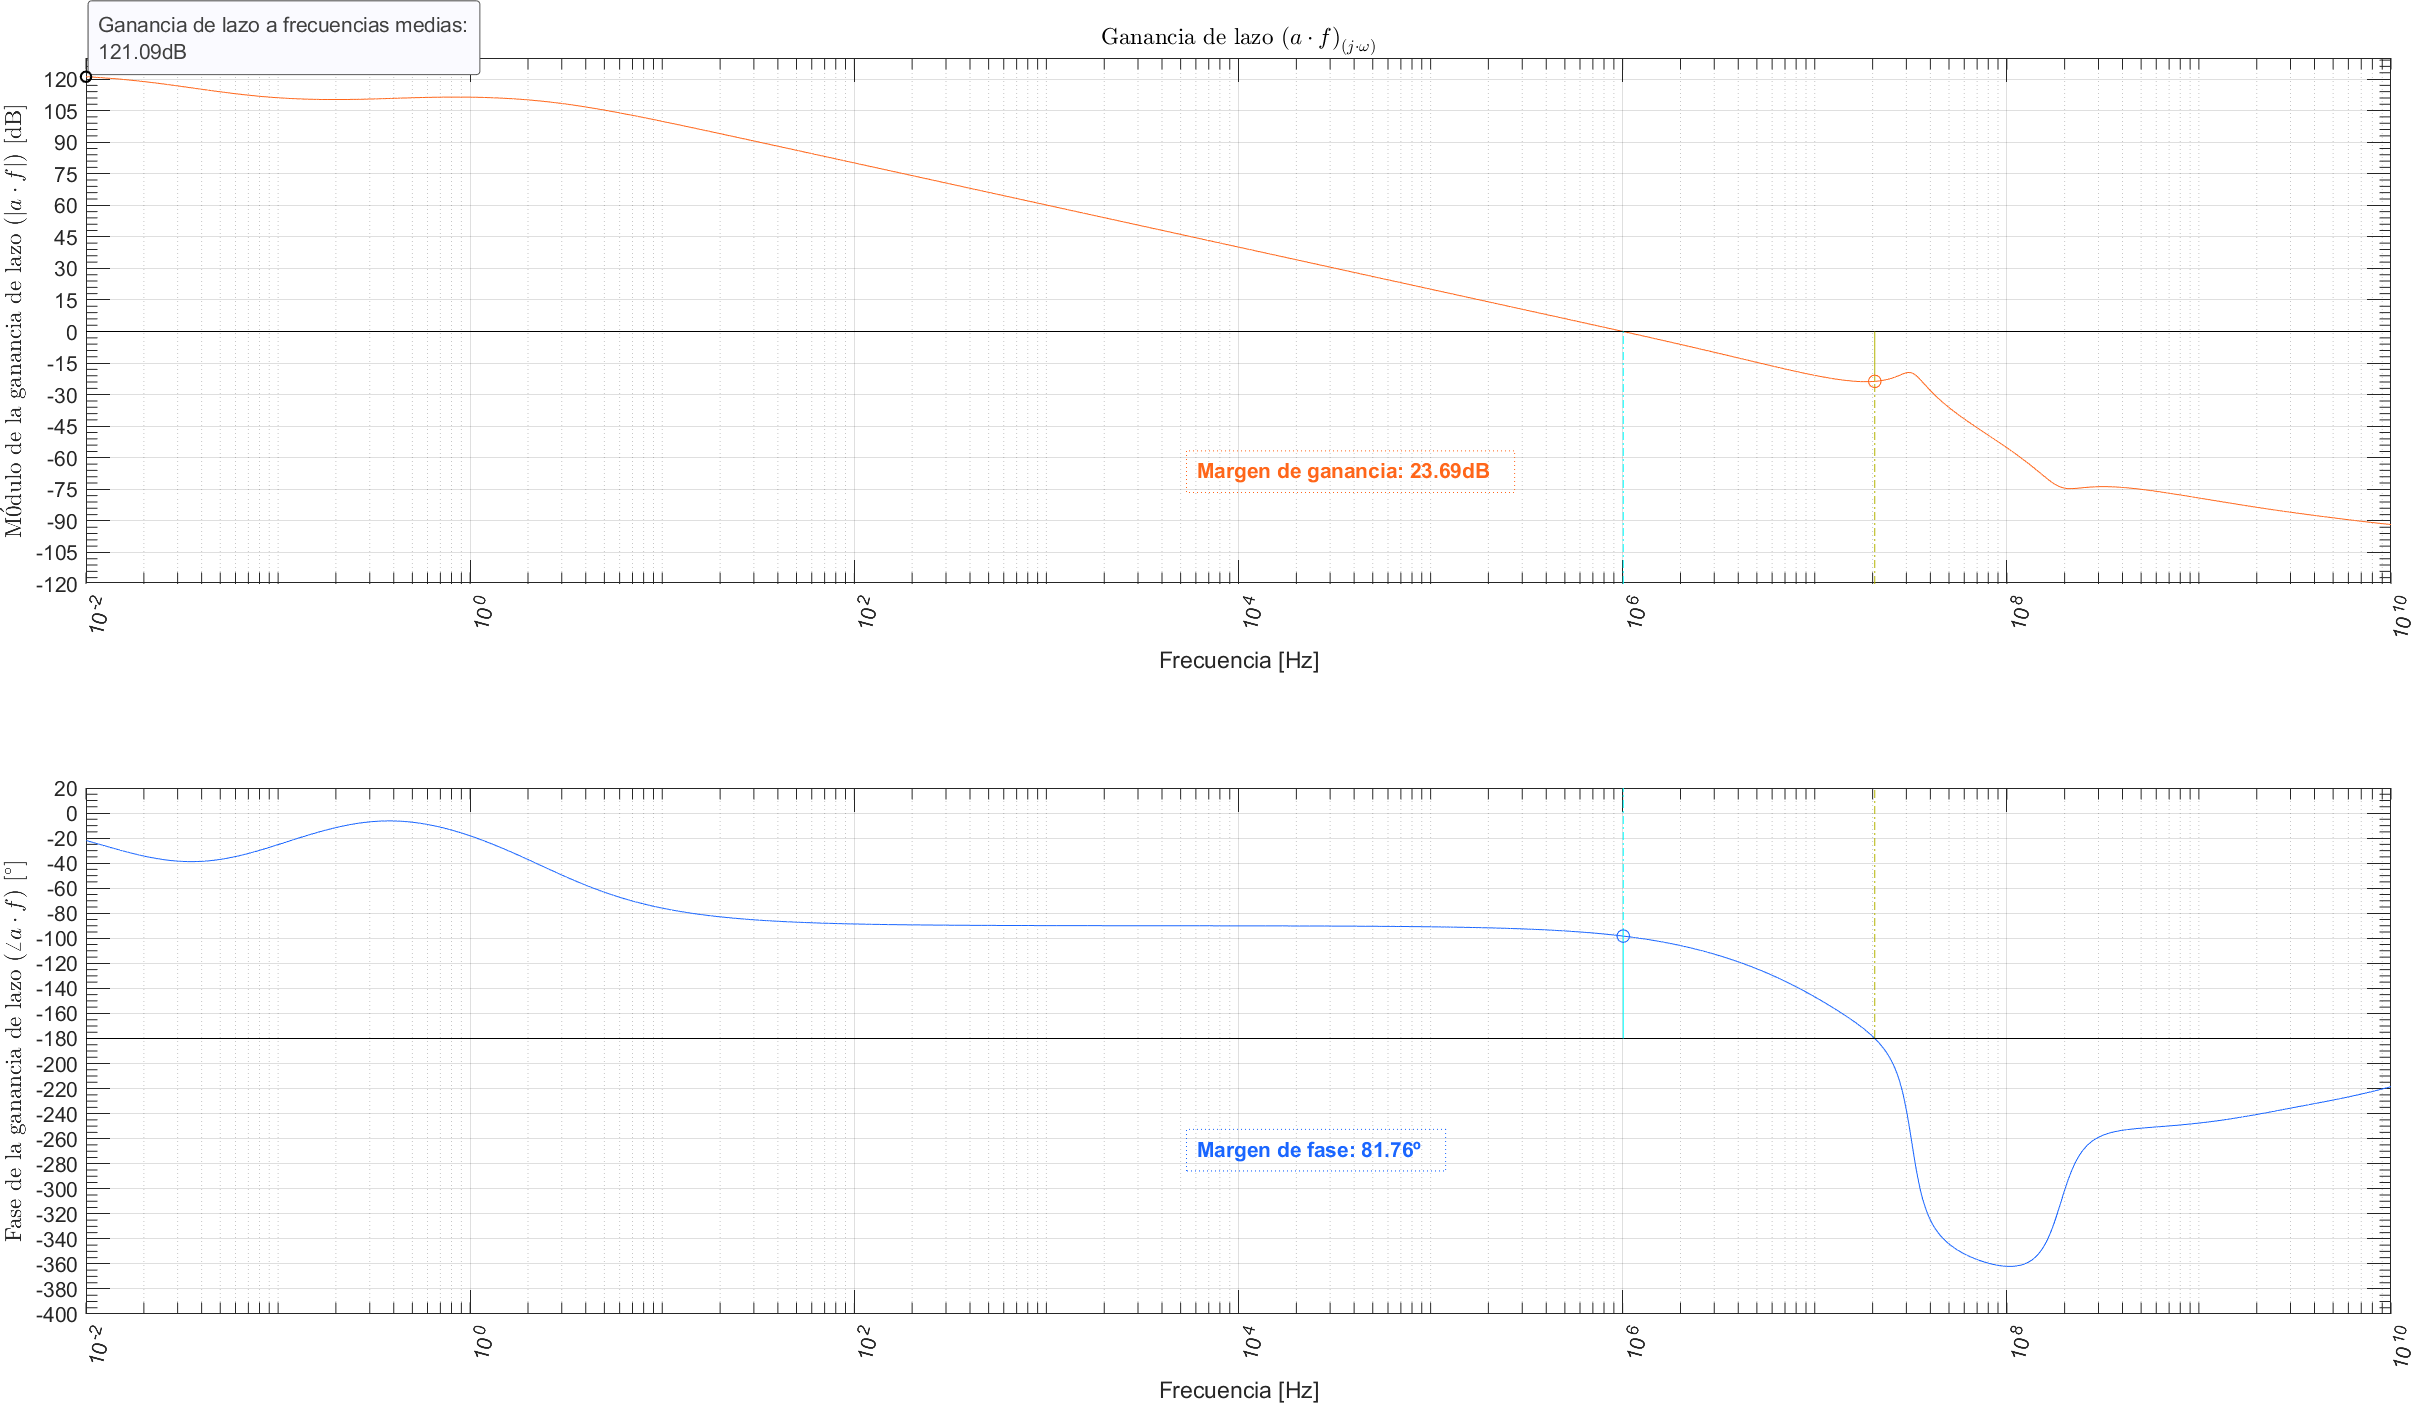
\includegraphics[width=0.93 \textheight, angle=90]{./img/simulaciones/Loop/gain_loop_2.png}
\caption{\label{fig:fig_loop_gain_2}\footnotesize{Ganancia de lazo en función de la frecuencia, indicando los márgenes obtenidos.}}
\end{center}
\end{figure}

\clearpage




\subsection{Análisis de los resultados obtenidos para el \textbf{THD}}

En ambos casos analizados para la compensación, el \textbf{THD} aumenta con la frecuencia, como se espera, esto es debido principalmente a la caída de la ganancia dela lazo, que hace menos efectiva la realimentación negativa, esto sucede por la caída de la ganancia de cada etapa, debida a su vez a la caída de la ganancia de los transistores con el aumento de la frecuencia, debido a los efectos reactivos parásitos de los mismos, que influyen mas a mayores frecuencias, y también a otros factores, como la caída del $\beta$ de los transistores. \\

Del mismo modo, como es de esperarse, para el caso de la etapa de salida funcionando en clase \textbf{A}, el \textbf{THD} es menor en ambas frecuencias evaluadas para ambos casos de compensación, esto se explica fundamentalmente por la ausencia de distorsión por cross-over, pero también a la menor modulación de $r_{o}$ en la etapa de salida. \\

También se observa que el \textbf{THD} es mayor en el caso de utilizarse un capacitor de compensación Miller de un orden de magnitud mayor, esto se explica principalmente por la caída de la ganancia de lazo que este capacitor produce, siendo mas evidente en este caso, que para el caso del capacitor de menor valor, el hecho de que el efecto sea mucho mayor a $10 \si[per-mode=symbol]{\kilo\hertz}$ que a $1 \si[per-mode=symbol]{\kilo\hertz}$, apoya esta justificación, a $1 \si[per-mode=symbol]{\kilo\hertz}$ el \textbf{THD} tiene un valor muy cercano al doble, mientras que a $10 \si[per-mode=symbol]{\kilo\hertz}$, el \textbf{THD} es unas \num{50} mas grande.









\clearpage
%\\\\\\\\\\\\\\\\\\\\\\\\\\\


%\\\\\\\\\\\\\\\\\\\\\\\\\\\
\section{Observaciones y conclusiones}
\resetallcounters

\subsection{Observaciones y conclusiones}

Los resultados obtenidos son razonables, al menos en forma relativa entre los casos analizados, la exactitud del \textbf{THD} calculado en cada caso, es dependiente del programa, y muy dependiente de los modelos específicos usados para los transistores, se intento usar para estos, los modelos proveídos por los fabricantes de cada dispositivo. Como ya se menciono antes, hay una cuestión con la definición de lo que es clase \textbf{A} en una etapa de salida del tipo push-pull, pero al margen de eso, el resultado esperado de que la distorsión sea menor para clase \textbf{A}, que para clase \textbf{B}, se cumple. \\
A pesar de tratarse de un circuito incompleto, faltando los circuitos completos de polarización, las protecciones, etc. Las simulaciones demuestran claramente que al menos la topología es un muy buen punto de partida para un amplificador de audio de muy buena calidad. En particular con el uso de mejores transistores para la etapa de salida, por ejemplo los transistores \textbf{TOSHIBA} que se mencionaron en clase, como algunas otras mejoras que se pueden introducir, como ser una carga activa para el par diferencial con mejor factor de copia y mayor resistencia de salida, o una etapa pre-driver a la salida, que presente al \textbf{VAS} una todavía mayor resistencia, un \textbf{VAS} cascode, etc. Son todas cosas que se pueden incorporar para mejorar aún mas la calidad del amplificador.

\cleardoublepage
%\\\\\\\\\\\\\\\\\\\\\\\\\\\


%\\\\\\\\\\\\\\\\\\\\\\\\\\\
%Reinicio la cuenta y seteo el estilo de headers y footers.
\pagestyle{bibliostyle}
%\\\\\\\\\\\\\\\\\\\\\\\\\\\

%\\\\\\\\\\\\\\\\\\\\\\\\\\\
\section{Bibliografía}
\resetallcounters

\begin{thebibliography}{9}




\bibitem{Gray_Meyer3}
\Needspace*{7\baselineskip}
\emph{Analysis and Design of Analog Integrated Circuits (3\textsuperscript{rd} Edition)}\\
Author: Paul R. Gray\\
Author: Robert G. Meyer\\
Publisher: John Wiley \& Sons, Inc.; 3\textsuperscript{rd} Edition (Janury 15, 1993)\\
Copyright: \textcopyright \space 1993, John Wiley \& Sons, Inc.\\
ISBN 10: 0471574953\\
Website: \weblink{http://www.wiley.com/WileyCDA/WileyTitle/productCd-EHEP000220.html}{Analysis and Design of Analog Integrated Circuits (3\textsuperscript{rd} Edition)}\\




\bibitem{Gray_Meyer4}
\Needspace*{10\baselineskip}
\emph{Analysis and Design of Analog Integrated Circuits (4\textsuperscript{th} Edition)}\\
Author: Paul R. Gray\\
Author: Paul J. Hurst\\
Author: Stephen H. Lewis\\
Author: Robert G. Meyer\\
Publisher: John Wiley \& Sons, Inc.; 4\textsuperscript{th} Edition (2001)\\
Copyright: \textcopyright \space 2001, John Wiley \& Sons, Inc.\\
ISBN 10: 0471321680\\
ISBN 13: 9780471321682\\
Website: \weblink{http://www.wiley.com/WileyCDA/WileyTitle/productCd-EHEP000220.html}{Analysis and Design of Analog Integrated Circuits (4\textsuperscript{th} Edition)}\\




\bibitem{Gray_Meyer5}
\Needspace*{10\baselineskip}
\emph{Analysis and Design of Analog Integrated Circuits (5\textsuperscript{th} Edition)}\\
Author: Paul R. Gray\\
Author: Paul J. Hurst\\
Author: Stephen H. Lewis\\
Author: Robert G. Meyer\\
Publisher: John Wiley \& Sons, Inc.; 5\textsuperscript{th} Edition (2009)\\
Copyright: \textcopyright \space 2001, John Wiley \& Sons, Inc.\\
ISBN 10: 0470245999\\
ISBN 13: 9780470245996\\
Website: \weblink{https://www.wiley.com/en-ar/Analysis+and+Design+of+Analog+Integrated+Circuits\%2C+5th+Edition-p-9780470245996}{Analysis and Design of Analog Integrated Circuits (5\textsuperscript{th} Edition)}\\



\bibitem{Sedra_Smith_ESP4}
\Needspace*{9\baselineskip}
\emph{Circuitos microelectrónicos (4\textsuperscript{ta} Edición) español}\\
Author: Adel. S. Sedra\\
Author: Kenneth C. Smith\\
Publisher: Oxford, University press; 4\textsuperscript{ta} Edición (2001)\\
Copyright: \textcopyright \space 1999, Oxford, University press México.\\
Original Copyright: \textcopyright \space 1998, 1991, 1987, 1982, Oxford, University press Inc.\\
ISBN 10: 01951166310\\
Website: \weblink{http://www.oup.com/us/companion.websites/0195142519/}{Circuitos microelectrónicos (4\textsuperscript{ta} Edición) español}\\




\bibitem{Sedra_Smith_ENG5}
\Needspace*{8\baselineskip}
\emph{Microelectronic circuits (5\textsuperscript{th} Edition)}\\
Author: Adel. S. Sedra\\
Author: Kenneth C. Smith\\
Publisher: Oxford, University press; 5\textsuperscript{th} Edition (2004)\\
Copyright: \textcopyright \space 2004, 1998, 1991, 1987, 1982, Oxford, University press Inc.\\
ISBN 10: 0195142527\\
Website: \weblink{http://www.oup.com/us/companion.websites/0195142519/}{Microelectronic circuits (5\textsuperscript{th} Edition)}\\





\end{thebibliography}
\cleardoublepage
%\\\\\\\\\\\\\\\\\\\\\\\\\\\

%\\\\\\\\\\\\\\\\\\\\\\\\\\\
%Seteo el stilo de headers y footers.
\pagestyle{allpages}
%\\\\\\\\\\\\\\\\\\\\\\\\\\\

\appendix


\appendixpage
\addappheadtotoc

%\\\\\\\\\\\\\\\\\\\\\\\\\\\






\section{Hojas de datos}



%*********************************************

\subsection{TL431}
\label{datasheet_TL431}
\emph{\textbf{TL431}}\\
\emph{Adjustable precision shunt regulator}\\
\vspace{5pt}
Manufacturer page:	\weblink{http://www.ti.com/product/TL431}{http://www.ti.com/product/TL431}\\

Manufacturer Datasheet:	\weblink{http://www.ti.com/lit/gpn/tl431}{http://www.ti.com/lit/gpn/tl431}\\


\subsection{TL082}
\label{datasheet_TL082}
\emph{\textbf{TL082}}\\
\emph{Dual High Slew Rate JFET-Input Operational Amplifier}\\
\vspace{5pt}
Manufacturer page:	\weblink{http://www.ti.com/product/TL082?keyMatch=TL082}{http://www.ti.com/product/TL082?keyMatch=TL082}\\

Manufacturer Datasheet:	\weblink{http://www.ti.com/lit/gpn/tl082}{http://www.ti.com/lit/gpn/tl082}\\


\subsection{BC548}
\label{datasheet_BC548}
\emph{\textbf{BC548}}\\
\emph{NPN Epitaxial Silicon Transistor}\\
\vspace{5pt}
Manufacturer page:	\weblink{https://www.onsemi.com/PowerSolutions/product.do?id=BC548}{https://www.onsemi.com/PowerSolutions/product.do?id=BC548}\\

Manufacturer Datasheet:	\weblink{https://www.onsemi.com/pub/Collateral/BC550-D.pdf}{https://www.onsemi.com/pub/Collateral/BC550-D.pdf}\\


\subsection{BC558}
\label{datasheet_BC558}
\emph{\textbf{BC558}}\\
\emph{PNP Bipolar Transistor}\\
\vspace{5pt}
Manufacturer page:	\weblink{https://www.onsemi.com/PowerSolutions/product.do?id=BC558B}{https://www.onsemi.com/PowerSolutions/product.do?id=BC558B}\\

Manufacturer Datasheet:	\weblink{https://www.onsemi.com/pub/Collateral/BC556B-D.PDF}{https://www.onsemi.com/pub/Collateral/BC556B-D.PDF}\\

\clearpage


\subsection{BD137}
\label{datasheet_BD137}
\emph{\textbf{BD137}}\\
\emph{$1.5 \si[per-mode=symbol]{\ampere}$, $60 \si[per-mode=symbol]{\volt}$ NPN Bipolar Power Transistor}\\
\vspace{5pt}
Manufacturer page:	\weblink{https://www.onsemi.com/PowerSolutions/product.do?id=BD137}{https://www.onsemi.com/PowerSolutions/product.do?id=BD137}\\

Manufacturer Datasheet:	\weblink{https://www.onsemi.com/pub/Collateral/BD135-D.PDF}{https://www.onsemi.com/pub/Collateral/BD135-D.PDF}\\


\subsection{MJE15032}
\label{datasheet_MJE15032}
\emph{\textbf{MJE15032}}\\
\emph{Bipolar Transistor, NPN, $250 \si[per-mode=symbol]{\volt}$, $8.0 \si[per-mode=symbol]{\ampere}$}\\
\vspace{5pt}
Manufacturer page:	\weblink{https://www.onsemi.com/PowerSolutions/product.do?id=MJE15032}{https://www.onsemi.com/PowerSolutions/product.do?id=MJE15032}\\

Manufacturer Datasheet:	\weblink{https://www.onsemi.com/pub/Collateral/MJE15032-D.PDF}{https://www.onsemi.com/pub/Collateral/MJE15032-D.PDF}\\


\subsection{MJE2955}
\label{datasheet_MJE2955}
\emph{\textbf{MJE2955}}\\
\emph{Bipolar Power Transistor, PNP, $10 \si[per-mode=symbol]{\ampere}$, $60 \si[per-mode=symbol]{\volt}$, $75 \si[per-mode=symbol]{\watt}$}\\
\vspace{5pt}
Manufacturer page:	\weblink{https://www.onsemi.com/PowerSolutions/product.do?id=MJE2955T}{https://www.onsemi.com/PowerSolutions/product.do?id=MJE2955T}\\

Manufacturer Datasheet:	\weblink{https://www.onsemi.com/pub/Collateral/MJE2955T-D.PDF}{hhttps://www.onsemi.com/pub/Collateral/MJE2955T-D.PDF}\\


\subsection{Metal film resistor}
\label{datasheet_METALFILMRESISTOR}
\emph{\textbf{Metal film resistor}}\\
\emph{Metal film resistor}\\
\vspace{5pt}
Manufacturer page:	\weblink{https://www.vishay.com/resistors-fixed/metal-film/tab/doclibrary/}{https://www.vishay.com/resistors-fixed/metal-film/tab/doclibrary/}\\



\subsection{Carbon film resistor}
\label{datasheet_CARBONFILMRESISTOR}
\emph{\textbf{Carbon film resistor}}\\
\emph{Carbon film resistor}\\
\vspace{5pt}
Manufacturer page:	\weblink{http://www.vishay.com/resistors-fixed/carbon-film/tab/doclibrary/}{http://www.vishay.com/resistors-fixed/carbon-film/tab/doclibrary/}\\


\clearpage


\subsection{Ceramic capacitor}
\label{datasheet_CERAMIC_CAPACITOR}
\emph{\textbf{Ceramic capacitor}}\\
\emph{Ceramic disk capacitor}\\
\vspace{5pt}
Manufacturer page:	\weblink{https://www.vishay.com/capacitors/ceramic/disc/}{https://www.vishay.com/capacitors/ceramic/disc/}\\


\subsection{Electrolitic Aluminum capacitor}
\label{datasheet_ELECTROLITIC_CAPACITOR}
\emph{\textbf{Electrolitic capacitor}}\\
\emph{Electrolitic aluminum capacitor}\\
\vspace{5pt}
Manufacturer page:	\weblink{https://www.vishay.com/capacitors/aluminum/}{https://www.vishay.com/capacitors/aluminum/}\\










\clearpage
%\\\\\\\\\\\\\\\\\\\\\\\\\\\

\end{document}
